\documentclass[aspectratio=169,11pt]{beamer}
\usetheme{metropolis}
\usepackage{tikz}
\usetikzlibrary{arrows.meta,positioning,decorations.pathmorphing,calc,shapes.geometric,decorations.pathreplacing,patterns}
\usepackage{pgfplots}
\pgfplotsset{compat=1.18}
\usepackage{booktabs}
\usepackage{xcolor}
\usepackage{amsmath,amssymb}
\usepackage{graphicx}
\usepackage{hyperref}
\hypersetup{colorlinks=true,urlcolor=grass,linkcolor=black,citecolor=black}
\usepackage{multirow}

\definecolor{grass}{HTML}{2E7D32}
\definecolor{circle}{HTML}{E91E63}
\definecolor{das}{HTML}{2196F3}
\definecolor{vae}{HTML}{9C27B0}
\definecolor{nldas}{HTML}{FF9800}
\definecolor{neutral}{HTML}{9E9E9E}
\definecolor{pass}{HTML}{4CAF50}
\definecolor{fail}{HTML}{F44336}
\definecolor{stoch}{HTML}{FF9800}
\definecolor{never}{HTML}{F44336}
\definecolor{always}{HTML}{4CAF50}
\definecolor{bg}{HTML}{FAFAFA}
\definecolor{memo}{HTML}{795548}

\newcommand{\Gr}{\mathrm{Gr}}
\newcommand{\IIA}{\mathrm{IIA}}
\newcommand{\R}{\mathbb{R}}
\newcommand{\Z}{\mathbb{Z}}

\title{When Does Linear Causal Abstraction Work?}
\subtitle{Mapping the boundary on the Grassmannian}
\author{Elliot Tower}
\date{2026}
\institute{}

\begin{document}

\maketitle

%% --- OVERVIEW ---
\begin{frame}{Overview}
\begin{columns}[T]
\begin{column}{0.32\textwidth}
\textbf{Part 1: Setup}
\begin{enumerate}
  \item What is a causal variable?
  \item DAS and the Grassmannian
  \item Why linearity matters
\end{enumerate}
\vspace{0.5em}
\textbf{Part 2: The atlas}
\begin{enumerate}
  \setcounter{enumi}{3}
  \item 14 operations, three classes
  \item Linear DAS fails completely
  \item Stochastic grokking
\end{enumerate}
\end{column}
\begin{column}{0.32\textwidth}
\textbf{Part 3: The vacuity problem}
\begin{enumerate}
  \setcounter{enumi}{6}
  \item Memorization artifacts
  \item NL-DAS is vacuous
  \item Intervention faithfulness
\end{enumerate}
\vspace{0.5em}
\textbf{Part 4: The fix}
\begin{enumerate}
  \setcounter{enumi}{9}
  \item Structured VAE
  \item Cross-task transfer
  \item IOI is not Grassmannian
\end{enumerate}
\end{column}
\begin{column}{0.32\textwidth}
\textbf{Part 5: Implications}
\begin{enumerate}
  \setcounter{enumi}{12}
  \item Four-level hierarchy
  \item Continuous metrics
  \item Practical advice
  \item Conclusion
\end{enumerate}
\end{column}
\end{columns}
\end{frame}

%% ============================================================
%% PART 1: SETUP
%% ============================================================

\begin{frame}[plain]
\vfill
\begin{center}
  \setlength{\fboxrule}{2.5pt}%
  \fcolorbox{black}{white}{\parbox{0.7\textwidth}{\centering\vspace{0.8em}
    {\Large\bfseries Part 1}\\[0.5em]
    {\large What is a causal variable, and where does DAS look?}
  \vspace{0.8em}}}
\end{center}
\vfill
\end{frame}

\begin{frame}{In this section}
\begin{columns}[T]
\begin{column}{0.48\textwidth}
\textbf{1. What is a causal variable?}\\[0.2em]
{\small When we say a neural network ``uses'' a concept, we mean there is a direction (or subspace) in its activations that, when edited, changes the output in a predictable way.}

\vspace{0.6em}
\textbf{2. DAS and the Grassmannian}\\[0.2em]
{\small Distributed Alignment Search (DAS) finds these subspaces. Every DAS solution is a point on a specific mathematical object: the Grassmannian manifold. This is the hidden assumption.}
\end{column}
\begin{column}{0.48\textwidth}
\textbf{3. Why linearity matters}\\[0.2em]
{\small DAS assumes the causal variable is a linear subspace. This works for some variables but fails catastrophically for others --- and high IIA scores cannot tell you which case you are in.}
\end{column}
\end{columns}
\end{frame}

\section{1. What is a causal variable?}

%% --- SLIDE: The interpretability goal ---
\begin{frame}{The interpretability goal}

{\small We want to understand \emph{how} neural networks compute, not just \emph{what} they compute.}

\vspace{0.5em}

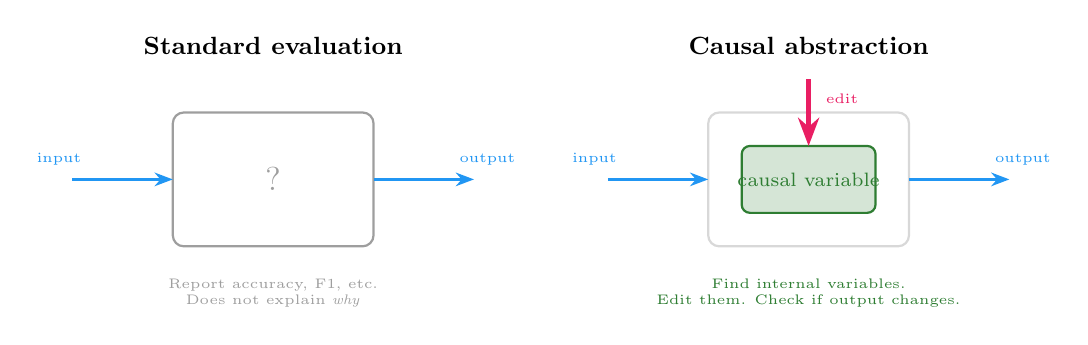
\begin{tikzpicture}[scale=0.85]
  % Left: black box
  \node[font=\small\bfseries] at (0,3.5) {Standard evaluation};
  \draw[neutral,thick,rounded corners=4pt] (-1.5,0.5) rectangle (1.5,2.5);
  \node[font=\large,neutral] at (0,1.5) {?};
  \draw[das,thick,-{Stealth}] (-3,1.5) -- (-1.5,1.5);
  \node[font=\tiny,das] at (-3.2,1.8) {input};
  \draw[das,thick,-{Stealth}] (1.5,1.5) -- (3,1.5);
  \node[font=\tiny,das] at (3.2,1.8) {output};
  \node[font=\tiny,neutral,align=center] at (0,-0.2) {Report accuracy, F1, etc.\\Does not explain \emph{why}};

  % Right: causal variable
  \node[font=\small\bfseries] at (8,3.5) {Causal abstraction};
  \draw[neutral!40,thick,rounded corners=4pt] (6.5,0.5) rectangle (9.5,2.5);
  \draw[das,thick,-{Stealth}] (5,1.5) -- (6.5,1.5);
  \node[font=\tiny,das] at (4.8,1.8) {input};
  \draw[das,thick,-{Stealth}] (9.5,1.5) -- (11,1.5);
  \node[font=\tiny,das] at (11.2,1.8) {output};

  % The causal variable inside
  \fill[grass!20,rounded corners=3pt] (7.0,1.0) rectangle (9.0,2.0);
  \draw[grass,thick,rounded corners=3pt] (7.0,1.0) rectangle (9.0,2.0);
  \node[font=\scriptsize,grass] at (8,1.5) {causal variable};

  % Edit arrow
  \draw[circle,ultra thick,-{Stealth}] (8,3.0) -- (8,2.0);
  \node[font=\tiny,circle] at (8.5,2.7) {edit};

  \node[font=\tiny,grass,align=center] at (8,-0.2) {Find internal variables.\\Edit them. Check if output changes.};
\end{tikzpicture}

\vspace{0.3em}
{\small If editing a specific direction in the network's internal representation changes the output predictably, that direction is a \textbf{causal variable} for the behavior.}
\end{frame}

%% --- SLIDE: Interchange intervention ---
\begin{frame}{Interchange intervention analysis (IIA)}

{\small The core technique: take two inputs, swap part of their internal representations, check if the output changes accordingly.}

\vspace{0.5em}

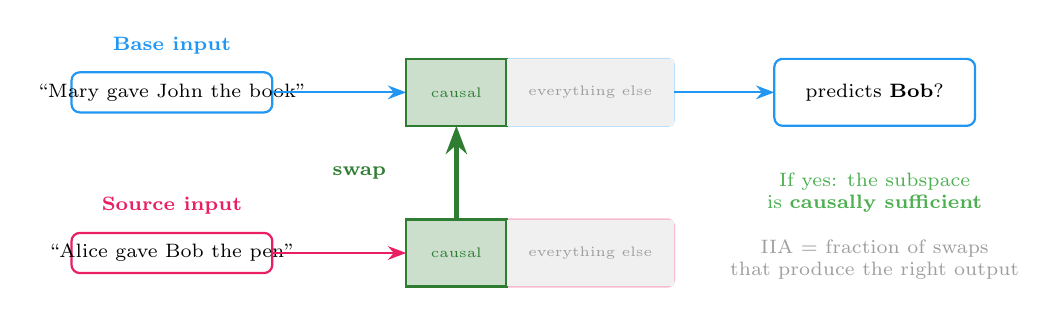
\begin{tikzpicture}[scale=0.85]
  % Base path
  \node[font=\scriptsize\bfseries,das] at (-0.5,4.2) {Base input};
  \draw[das,thick,rounded corners=3pt] (-2,3.2) rectangle (1,3.8);
  \node[font=\scriptsize] at (-0.5,3.5) {``Mary gave John the book''};

  % Source path
  \node[font=\scriptsize\bfseries,circle] at (-0.5,1.8) {Source input};
  \draw[circle,thick,rounded corners=3pt] (-2,0.8) rectangle (1,1.4);
  \node[font=\scriptsize] at (-0.5,1.1) {``Alice gave Bob the pen''};

  % Activations
  \draw[das,thick,-{Stealth}] (1,3.5) -- (3,3.5);
  \draw[circle,thick,-{Stealth}] (1,1.1) -- (3,1.1);

  % Activation boxes
  \draw[das!30,thick,rounded corners=2pt] (3,3.0) rectangle (7,4.0);
  \fill[grass!25] (3,3.0) rectangle (4.5,4.0);
  \draw[grass,thick] (3,3.0) rectangle (4.5,4.0);
  \node[font=\tiny,grass] at (3.75,3.5) {causal};
  \fill[neutral!15] (4.5,3.0) rectangle (7,4.0);
  \node[font=\tiny,neutral] at (5.75,3.5) {everything else};

  \draw[circle!30,thick,rounded corners=2pt] (3,0.6) rectangle (7,1.6);
  \fill[grass!25] (3,0.6) rectangle (4.5,1.6);
  \draw[grass,thick] (3,0.6) rectangle (4.5,1.6);
  \node[font=\tiny,grass] at (3.75,1.1) {causal};
  \fill[neutral!15] (4.5,0.6) rectangle (7,1.6);
  \node[font=\tiny,neutral] at (5.75,1.1) {everything else};

  % Swap arrow
  \draw[grass,ultra thick,-{Stealth}] (3.75,1.6) -- (3.75,3.0);
  \node[font=\scriptsize\bfseries,grass] at (2.3,2.3) {swap};

  % Output
  \draw[das,thick,-{Stealth}] (7,3.5) -- (8.5,3.5);
  \draw[das,thick,rounded corners=3pt] (8.5,3.0) rectangle (11.5,4.0);
  \node[font=\scriptsize,align=center] at (10,3.5) {predicts \textbf{Bob}?};

  % IIA label
  \node[font=\scriptsize,pass,align=center] at (10,2.0) {If yes: the subspace\\is \textbf{causally sufficient}};
  \node[font=\scriptsize,neutral,align=center] at (10,1.0) {IIA = fraction of swaps\\that produce the right output};
\end{tikzpicture}
\end{frame}

\section{2. DAS and the Grassmannian}

%% --- SLIDE: What DAS actually does ---
\begin{frame}{What DAS actually does}

\begin{columns}[T]
\begin{column}{0.55\textwidth}
{\small DAS learns a rotation matrix $Q \in \R^{d \times k}$ that identifies a $k$-dimensional subspace of the $d$-dimensional activation space.}

\vspace{0.3em}
{\small The interchange intervention projects out the base's component and replaces it with the source's:}

$$h' = h_b - QQ^\top h_b + QQ^\top h_s$$

{\small This is a \textbf{linear} operation. The subspace $QQ^\top$ is an orthogonal projection onto a \emph{flat plane} in activation space.}

\vspace{0.3em}
{\small The set of all $k$-dimensional planes in $\R^d$ is the \textbf{Grassmannian manifold} $\Gr(k,d)$.}

\vspace{0.3em}
{\small Every DAS solution is a point on $\Gr(k,d)$.}
\end{column}
\begin{column}{0.42\textwidth}
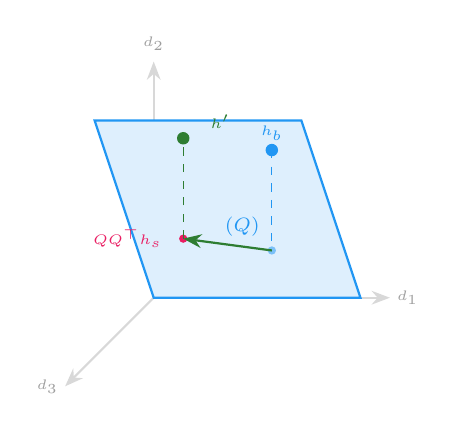
\begin{tikzpicture}[scale=0.75]
  % 3D-ish activation space
  \draw[neutral!40,thick,-{Stealth}] (0,0) -- (4,0);
  \draw[neutral!40,thick,-{Stealth}] (0,0) -- (0,4);
  \draw[neutral!40,thick,-{Stealth}] (0,0) -- (-1.5,-1.5);
  \node[font=\tiny,neutral] at (4.3,0) {$d_1$};
  \node[font=\tiny,neutral] at (0,4.3) {$d_2$};
  \node[font=\tiny,neutral] at (-1.8,-1.5) {$d_3$};

  % The subspace (a plane)
  \fill[das!15] (0,0) -- (3.5,0) -- (2.5,3) -- (-1,3) -- cycle;
  \draw[das,thick] (0,0) -- (3.5,0) -- (2.5,3) -- (-1,3) -- cycle;
  \node[font=\scriptsize,das] at (1.5,1.2) {$\Span(Q)$};

  % Base point
  \fill[das] (2,2.5) circle (3pt);
  \node[font=\tiny,das,above] at (2,2.5) {$h_b$};

  % Projection
  \draw[das,dashed] (2,2.5) -- (2,0.8);
  \fill[das!60] (2,0.8) circle (2pt);

  % Source projection
  \fill[circle] (0.5,1.0) circle (2pt);
  \node[font=\tiny,circle,left] at (0.3,1.0) {$QQ^\top h_s$};

  % Intervened point
  \draw[grass,thick,-{Stealth}] (2,0.8) -- (0.5,1.0);
  \fill[grass] (2,2.5) ++(-1.5,0.2) circle (3pt);
  \node[font=\tiny,grass,above right] at (0.8,2.7) {$h'$};
  \draw[grass,dashed] (0.5,1.0) -- (0.5,2.7);
\end{tikzpicture}

\vspace{0.3em}
\centering
{\scriptsize DAS projects onto a \textbf{flat plane}.\\What if the variable lives on a \textbf{curve}?}
\end{column}
\end{columns}
\end{frame}

%% --- SLIDE: The Grassmannian ---
\begin{frame}{The Grassmannian manifold $\Gr(k,d)$}

\begin{columns}[T]
\begin{column}{0.55\textwidth}
{\small The Grassmannian $\Gr(k,d)$ is the set of all $k$-dimensional linear subspaces of $\R^d$.}

\vspace{0.3em}
{\small Think of it as a ``space of planes.'' Every DAS solution picks one plane from this space. The distance between two planes is measured by their \textbf{principal angles}:}

$$d_{\Gr}([Q_1],[Q_2]) = \left(\sum_i \theta_i^2\right)^{1/2}$$

{\small When we ask ``does DAS work?'' we are really asking:}

\vspace{0.3em}
\begin{center}
\fcolorbox{grass}{grass!10}{\parbox{0.85\linewidth}{\centering\vspace{0.3em}
  {\small Does the true causal variable live on $\Gr(k,d)$?}
\vspace{0.3em}}}
\end{center}

\vspace{0.3em}
{\small If yes: DAS finds a meaningful point.\\
If no: DAS still returns a point, but it is an \textbf{artifact}.}
\end{column}
\begin{column}{0.42\textwidth}
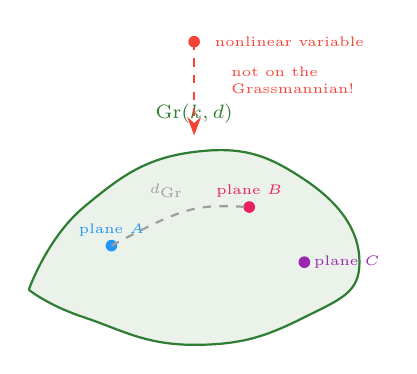
\begin{tikzpicture}[scale=0.7]
  % Grassmannian as a curved surface
  \draw[grass,thick,fill=grass!10]
    plot[smooth,tension=0.8] coordinates {(-2,0) (-1,1.5) (1,2.5) (3,2) (4,0.5) (3,-0.5) (1,-1) (-1,-0.5) (-2,0)};
  \node[font=\scriptsize\bfseries,grass] at (1,3.2) {$\Gr(k,d)$};

  % Points on it = different subspaces
  \fill[das] (-0.5,0.8) circle (3pt);
  \node[font=\tiny,das,above] at (-0.5,0.8) {plane $A$};

  \fill[circle] (2,1.5) circle (3pt);
  \node[font=\tiny,circle,above] at (2,1.5) {plane $B$};

  \fill[vae] (3,0.5) circle (3pt);
  \node[font=\tiny,vae,right] at (3,0.5) {plane $C$};

  % Geodesic
  \draw[neutral,thick,dashed]
    plot[smooth,tension=0.6] coordinates {(-0.5,0.8) (0.5,1.3) (1.2,1.5) (2,1.5)};
  \node[font=\tiny,neutral] at (0.5,1.8) {$d_{\Gr}$};

  % Off-manifold point
  \fill[never] (1,4.5) circle (3pt);
  \node[font=\tiny,never,right] at (1.2,4.5) {nonlinear variable};
  \draw[never,thick,dashed,-{Stealth}] (1,4.5) -- (1,2.8);
  \node[font=\tiny,never,right,align=left] at (1.5,3.8) {not on the\\Grassmannian!};
\end{tikzpicture}

\vspace{0.5em}
\centering
{\scriptsize A nonlinear causal variable (circle, sphere)\\does not live on $\Gr(k,d)$ at any $k$.}
\end{column}
\end{columns}
\end{frame}

\section{3. Why linearity matters}

%% --- SLIDE: Linear vs nonlinear causal variables ---
\begin{frame}{Linear vs.\ nonlinear causal variables}

\begin{columns}[T]
\begin{column}{0.48\textwidth}
\centering
\textbf{\textcolor{das}{Linear causal variable}}

\vspace{0.3em}
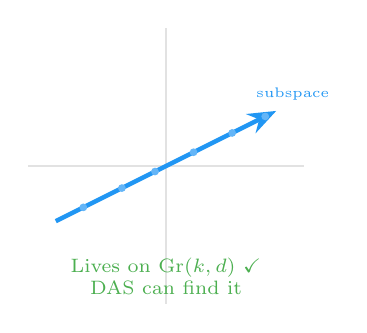
\begin{tikzpicture}[scale=0.7]
  \draw[neutral!30] (-2.5,0) -- (2.5,0);
  \draw[neutral!30] (0,-2.5) -- (0,2.5);

  % Linear subspace
  \draw[das,ultra thick,-{Stealth}] (-2,-1) -- (2,1);
  \node[font=\tiny,das] at (2.3,1.3) {subspace};

  % Points projected onto line
  \foreach \x/\y in {-1.5/-0.75, -0.8/-0.4, -0.2/-0.1, 0.5/0.25, 1.2/0.6, 1.8/0.9} {
    \fill[das!70] (\x,\y) circle (2pt);
  }

  \node[font=\scriptsize,pass,align=center] at (0,-2) {Lives on $\Gr(k,d)$ \checkmark\\DAS can find it};
\end{tikzpicture}

\vspace{0.3em}
{\small Examples: IOI indirect object (partially), multiplication mod $p$ after grokking}
\end{column}
\begin{column}{0.48\textwidth}
\centering
\textbf{\textcolor{circle}{Nonlinear causal variable}}

\vspace{0.3em}
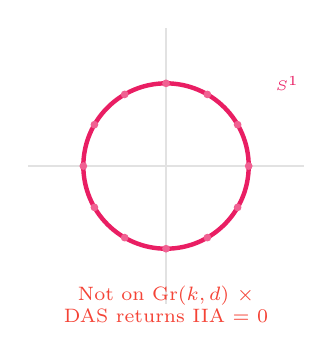
\begin{tikzpicture}[scale=0.7]
  \draw[neutral!30] (-2.5,0) -- (2.5,0);
  \draw[neutral!30] (0,-2.5) -- (0,2.5);

  % Circle
  \draw[circle,ultra thick] (0,0) circle (1.5);

  % Points on circle
  \foreach \a in {0,30,...,330} {
    \fill[circle!70] ({1.5*cos(\a)},{1.5*sin(\a)}) circle (2pt);
  }
  \node[font=\tiny,circle] at (2.2,1.5) {$S^1$};

  \node[font=\scriptsize,fail,align=center] at (0,-2.5) {Not on $\Gr(k,d)$ $\times$\\DAS returns IIA = 0};
\end{tikzpicture}

\vspace{0.3em}
{\small Examples: addition mod $p$ after grokking (Fourier representation encodes numbers on a circle)}
\end{column}
\end{columns}
\end{frame}

%% --- SLIDE: The central question ---
\begin{frame}{The central question}

\begin{center}
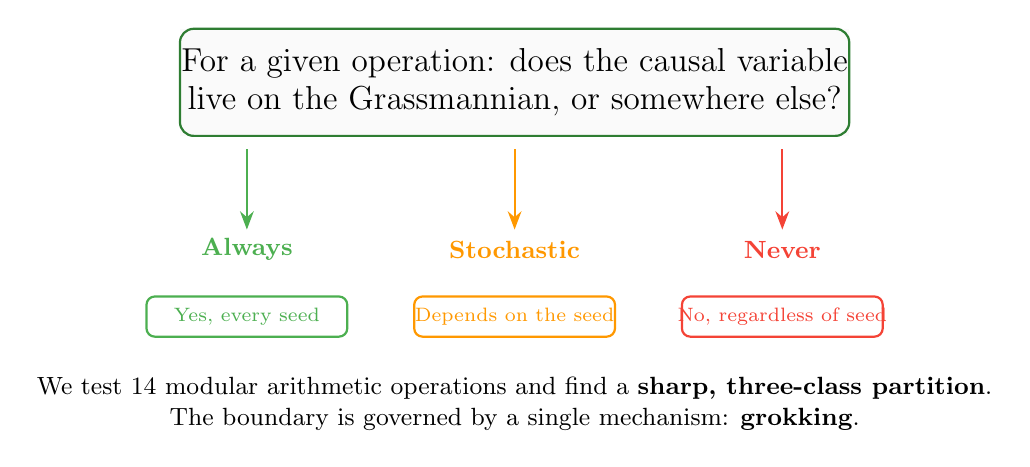
\begin{tikzpicture}[scale=0.85]
  % Question box
  \fill[bg] (-5,-0.8) rectangle (5,0.8);
  \draw[grass,thick,rounded corners=5pt] (-5,-0.8) rectangle (5,0.8);
  \node[font=\large,align=center] at (0,0) {For a given operation: does the causal variable\\live on the Grassmannian, or somewhere else?};

  % Three possibilities
  \node[font=\small\bfseries,always] at (-4,-2.5) {Always};
  \draw[always,thick,rounded corners=3pt] (-5.5,-3.2) rectangle (-2.5,-3.8);
  \node[font=\scriptsize,always,align=center] at (-4,-3.5) {Yes, every seed};

  \node[font=\small\bfseries,stoch] at (0,-2.5) {Stochastic};
  \draw[stoch,thick,rounded corners=3pt] (-1.5,-3.2) rectangle (1.5,-3.8);
  \node[font=\scriptsize,stoch,align=center] at (0,-3.5) {Depends on the seed};

  \node[font=\small\bfseries,never] at (4,-2.5) {Never};
  \draw[never,thick,rounded corners=3pt] (2.5,-3.2) rectangle (5.5,-3.8);
  \node[font=\scriptsize,never,align=center] at (4,-3.5) {No, regardless of seed};

  % Arrows
  \draw[always,thick,-{Stealth}] (-4,-1.0) -- (-4,-2.2);
  \draw[stoch,thick,-{Stealth}] (0,-1.0) -- (0,-2.2);
  \draw[never,thick,-{Stealth}] (4,-1.0) -- (4,-2.2);

  % Bottom line
  \node[font=\small,align=center] at (0,-4.8) {We test 14 modular arithmetic operations and find a \textbf{sharp, three-class partition}.\\The boundary is governed by a single mechanism: \textbf{grokking}.};
\end{tikzpicture}
\end{center}
\end{frame}


%% ============================================================
%% PART 2: THE ATLAS
%% ============================================================

\begin{frame}[plain]
\vfill
\begin{center}
  \setlength{\fboxrule}{2.5pt}%
  \fcolorbox{black}{white}{\parbox{0.7\textwidth}{\centering\vspace{0.8em}
    {\Large\bfseries Part 2}\\[0.5em]
    {\large The atlas: 14 operations, three classes}
  \vspace{0.8em}}}
\end{center}
\vfill
\end{frame}

\section{4. 14 operations, three classes}

%% --- SLIDE: Experimental setup ---
\begin{frame}{Experimental setup}

\begin{columns}[T]
\begin{column}{0.55\textwidth}
{\small We train single-layer transformers on modular arithmetic:}

\vspace{0.2em}
{\small Input: $(a, b, {=})$ \quad Output: $f(a,b) \bmod p$}

\vspace{0.3em}
{\small Model: $d_\text{model} = 128$, 4 heads, standard grokking setup (30\% train, AdamW, weight decay 1.0).}

\vspace{0.3em}
{\small For each trained model, we:}
\begin{enumerate}
  \item {\small Cache residual-stream activations}
  \item {\small Train DAS at $k \in \{2, 4, 6, \ldots, 32\}$}
  \item {\small Measure IIA, equivariance, circle geometry}
  \item {\small Train a structured VAE}
\end{enumerate}

\vspace{0.3em}
{\small 14 operations spanning group actions, polynomials, piecewise, and non-algebraic maps.}
\end{column}
\begin{column}{0.42\textwidth}
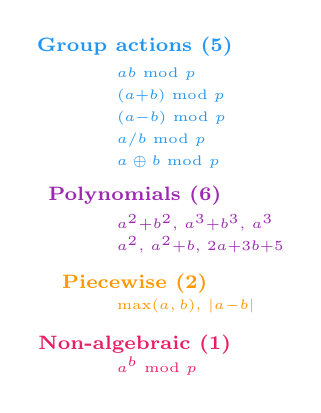
\begin{tikzpicture}[scale=0.7]
  % Operation categories
  \node[font=\scriptsize\bfseries,das] at (0,5.5) {Group actions (5)};
  \node[font=\tiny,das,anchor=west] at (-0.5,5.0) {$ab$ mod $p$};
  \node[font=\tiny,das,anchor=west] at (-0.5,4.6) {$(a{+}b)$ mod $p$};
  \node[font=\tiny,das,anchor=west] at (-0.5,4.2) {$(a{-}b)$ mod $p$};
  \node[font=\tiny,das,anchor=west] at (-0.5,3.8) {$a/b$ mod $p$};
  \node[font=\tiny,das,anchor=west] at (-0.5,3.4) {$a \oplus b$ mod $p$};

  \node[font=\scriptsize\bfseries,vae] at (0,2.8) {Polynomials (6)};
  \node[font=\tiny,vae,anchor=west] at (-0.5,2.3) {$a^2{+}b^2$, $a^3{+}b^3$, $a^3$};
  \node[font=\tiny,vae,anchor=west] at (-0.5,1.9) {$a^2$, $a^2{+}b$, $2a{+}3b{+}5$};

  \node[font=\scriptsize\bfseries,nldas] at (0,1.2) {Piecewise (2)};
  \node[font=\tiny,nldas,anchor=west] at (-0.5,0.8) {$\max(a,b)$, $|a{-}b|$};

  \node[font=\scriptsize\bfseries,circle] at (0,0.1) {Non-algebraic (1)};
  \node[font=\tiny,circle,anchor=west] at (-0.5,-0.3) {$a^b$ mod $p$};
\end{tikzpicture}
\end{column}
\end{columns}
\end{frame}

%% --- SLIDE: What is grokking ---
\begin{frame}{What is grokking?}

\begin{columns}[T]
\begin{column}{0.55\textwidth}
{\small \textbf{Grokking} is a training phenomenon where models memorize the training set long before they generalize.}

\vspace{0.3em}
{\small For modular arithmetic with weight decay:}
\begin{itemize}
  \item {\small Train loss drops to zero quickly (memorization)}
  \item {\small Test loss stays high for thousands of epochs}
  \item {\small Then suddenly drops (generalization)}
\end{itemize}

\vspace{0.3em}
{\small The internal representation changes during grokking: from a lookup table (memorization) to a structured algorithm (Fourier representation).}

\vspace{0.3em}
{\small Prior work showed grokked models use Fourier features:\\$a \mapsto (\cos 2\pi f a / p, \sin 2\pi f a / p)$}

\vspace{0.3em}
{\small Our contribution: \textbf{grokking determines whether the causal variable is Grassmannian.}}
\end{column}
\begin{column}{0.42\textwidth}
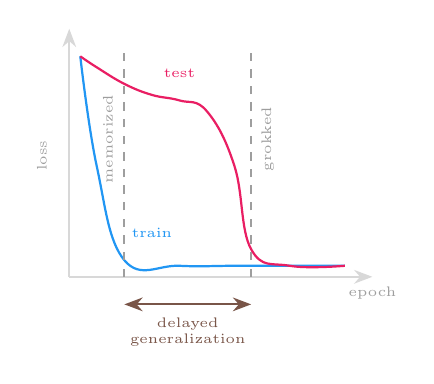
\begin{tikzpicture}[scale=0.7]
  % Training curve
  \draw[neutral!40,thick,-{Stealth}] (0,0) -- (5.5,0);
  \draw[neutral!40,thick,-{Stealth}] (0,0) -- (0,4.5);
  \node[font=\tiny,neutral] at (5.5,-0.3) {epoch};
  \node[font=\tiny,neutral,rotate=90] at (-0.5,2.2) {loss};

  % Train loss
  \draw[das,thick] plot[smooth,tension=0.7] coordinates {(0.2,4) (0.5,2) (1,0.3) (2,0.2) (3,0.2) (4,0.2) (5,0.2)};
  \node[font=\tiny,das] at (1.5,0.8) {train};

  % Test loss (grokking)
  \draw[circle,thick] plot[smooth,tension=0.7] coordinates {(0.2,4) (0.5,3.8) (1,3.5) (1.5,3.3) (2,3.2) (2.5,3.0) (3,2) (3.3,0.5) (4,0.2) (5,0.2)};
  \node[font=\tiny,circle] at (2,3.7) {test};

  % Annotations
  \draw[neutral,thick,dashed] (1,0) -- (1,4.2);
  \node[font=\tiny,neutral,align=center,rotate=90] at (0.7,2.5) {memorized};

  \draw[neutral,thick,dashed] (3.3,0) -- (3.3,4.2);
  \node[font=\tiny,neutral,align=center,rotate=90] at (3.6,2.5) {grokked};

  % Phase labels
  \draw[{Stealth}-{Stealth},memo,thick] (1,-0.5) -- (3.3,-0.5);
  \node[font=\tiny,memo,align=center] at (2.15,-1.0) {delayed\\generalization};
\end{tikzpicture}
\end{column}
\end{columns}
\end{frame}

%% --- SLIDE: The atlas results ---
\begin{frame}{The atlas: three sharp classes}
\centering
\vspace{-0.3em}
{\small\setlength{\tabcolsep}{3pt}
\begin{tabular}{lcccccl}
\toprule
\textbf{Operation} & \textbf{Grok} & \textbf{Loss} & \textbf{IIA}($k{=}2$) & $\boldsymbol{k^*}$ & \textbf{Equiv.} & \textbf{Class} \\
\midrule
Multiplication & \checkmark & 0.000 & 1.000 & 2 & 0.995 & \textcolor{always}{Always} \\
Subtraction & \checkmark & 0.000 & 1.000 & 2 & 1.000 & \textcolor{always}{Always} \\
Division & \checkmark & 0.000 & 1.000 & 2 & 1.000 & \textcolor{always}{Always} \\
Bitwise XOR & \checkmark & 0.003 & 1.000 & 2 & 1.000 & \textcolor{always}{Always} \\
Cubic sum & \checkmark & 0.000 & 1.000 & 2 & 1.000 & \textcolor{always}{Always} \\
Sum of squares & \checkmark & 0.005 & 1.000 & 2 & 0.987 & \textcolor{always}{Always} \\
Max & \checkmark & 0.074 & 0.960 & 2 & 0.957 & \textcolor{always}{Always} \\
\midrule
Power (s137) & \checkmark & 0.088 & 0.940 & 4 & 0.965 & \textcolor{stoch}{Stochastic} \\
Power (s42) & $\times$ & 1.143 & 0.980 & 2 & 0.665 & \textcolor{stoch}{Stochastic} \\
\midrule
Cubing & $\times$ & 9.765 & 0.857 & 4 & 0.509 & \textcolor{never}{Never} \\
Squaring & $\times$ & 7.808 & 0.857 & 4 & 0.314 & \textcolor{never}{Never} \\
Abs.\ difference & $\times$ & 1.835 & 0.800 & ${>}32$ & 0.189 & \textcolor{never}{Never} \\
Polynomial & $\times$ & 21.55 & 0.720 & ${>}32$ & 0.015 & \textcolor{never}{Never} \\
Affine & $\times$ & 26.21 & 0.780 & ${>}32$ & 0.026 & \textcolor{never}{Never} \\
\bottomrule
\end{tabular}}

\vspace{0.3em}
{\small $k^*$ = smallest $k$ where IIA $\geq 0.95$. Equiv.\ = equivariance under additive shift.}
\end{frame}

%% --- SLIDE: Visual summary of classes ---
\begin{frame}{Three classes, one mechanism}

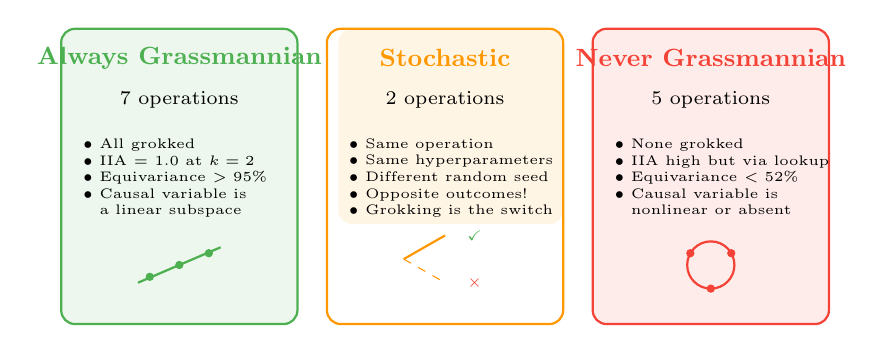
\begin{tikzpicture}[scale=0.75]
  % Always
  \fill[always!10,rounded corners=5pt] (-5.5,-0.5) rectangle (-1.5,4.5);
  \draw[always,thick,rounded corners=5pt] (-5.5,-0.5) rectangle (-1.5,4.5);
  \node[font=\small\bfseries,always] at (-3.5,4.0) {Always Grassmannian};
  \node[font=\scriptsize,align=center] at (-3.5,3.3) {7 operations};
  \node[font=\tiny,align=left,anchor=north west] at (-5.3,2.8) {%
    $\bullet$ All grokked\\
    $\bullet$ IIA = 1.0 at $k = 2$\\
    $\bullet$ Equivariance $> 95\%$\\
    $\bullet$ Causal variable is\\
    \phantom{$\bullet$} a linear subspace};
  % Mini diagram
  \draw[always,thick] (-4.2,0.2) -- (-2.8,0.8);
  \fill[always] (-4.0,0.3) circle (2pt);
  \fill[always] (-3.5,0.5) circle (2pt);
  \fill[always] (-3.0,0.7) circle (2pt);

  % Stochastic
  \fill[stoch!10,rounded corners=5pt] (-1,,-0.5) rectangle (3,4.5);
  \draw[stoch,thick,rounded corners=5pt] (-1,-0.5) rectangle (3,4.5);
  \node[font=\small\bfseries,stoch] at (1,4.0) {Stochastic};
  \node[font=\scriptsize,align=center] at (1,3.3) {2 operations};
  \node[font=\tiny,align=left,anchor=north west] at (-0.8,2.8) {%
    $\bullet$ Same operation\\
    $\bullet$ Same hyperparameters\\
    $\bullet$ Different random seed\\
    $\bullet$ Opposite outcomes!\\
    $\bullet$ Grokking is the switch};
  % Mini diagram: coin flip
  \draw[stoch,thick] (0.3,0.6) -- (1,1.0);
  \draw[stoch,dashed] (0.3,0.6) -- (1,0.2);
  \node[font=\tiny,always] at (1.5,1.0) {\checkmark};
  \node[font=\tiny,never] at (1.5,0.2) {$\times$};

  % Never
  \fill[never!10,rounded corners=5pt] (3.5,-0.5) rectangle (7.5,4.5);
  \draw[never,thick,rounded corners=5pt] (3.5,-0.5) rectangle (7.5,4.5);
  \node[font=\small\bfseries,never] at (5.5,4.0) {Never Grassmannian};
  \node[font=\scriptsize,align=center] at (5.5,3.3) {5 operations};
  \node[font=\tiny,align=left,anchor=north west] at (3.7,2.8) {%
    $\bullet$ None grokked\\
    $\bullet$ IIA high but via lookup\\
    $\bullet$ Equivariance $< 52\%$\\
    $\bullet$ Causal variable is\\
    \phantom{$\bullet$} nonlinear or absent};
  % Mini diagram: circle
  \draw[never,thick] (5.5,0.5) circle (0.4);
  \fill[never] ({5.5+0.4*cos(30)},{0.5+0.4*sin(30)}) circle (2pt);
  \fill[never] ({5.5+0.4*cos(150)},{0.5+0.4*sin(150)}) circle (2pt);
  \fill[never] ({5.5+0.4*cos(270)},{0.5+0.4*sin(270)}) circle (2pt);
\end{tikzpicture}
\end{frame}

\section{5. Linear DAS fails completely}

%% --- SLIDE: DAS = 0 on addition ---
\begin{frame}{Linear DAS returns zero IIA on grokked modular addition}

\begin{columns}[T]
\begin{column}{0.55\textwidth}
{\small Addition mod 113 groks perfectly (test loss $< 10^{-7}$). The model has learned the correct algorithm.}

\vspace{0.3em}
{\small But DAS returns $\IIA = 0.0$ at \textbf{every} subspace dimension $k \in \{2, 4, 8, 16\}$.}

\vspace{0.3em}
{\small This is not an optimization failure. The model encodes numbers using Fourier features:}

$$a \mapsto (\cos \tfrac{2\pi f a}{p}, \sin \tfrac{2\pi f a}{p})$$

{\small This representation lives on a \textbf{circle} $S^1$ embedded in $\R^d$, not on a linear subspace.}

\vspace{0.3em}
{\small DAS searches $\Gr(k,d)$ for a flat plane that captures a curved manifold --- a \textbf{category error}, not an optimization failure.}
\end{column}
\begin{column}{0.42\textwidth}
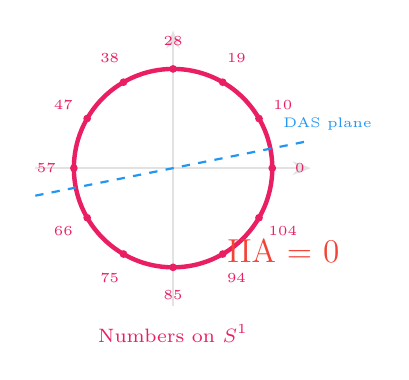
\begin{tikzpicture}[scale=0.7]
  % Circle in activation space
  \draw[neutral!30,thick,-{Stealth}] (-2.5,0) -- (2.5,0);
  \draw[neutral!30,thick,-{Stealth}] (0,-2.5) -- (0,2.5);

  % The circle
  \draw[circle,ultra thick] (0,0) circle (1.8);

  % Points labeled with numbers
  \foreach \a/\lab in {0/0, 30/10, 60/19, 90/28, 120/38, 150/47, 180/57, 210/66, 240/75, 270/85, 300/94, 330/104} {
    \fill[circle] ({1.8*cos(\a)},{1.8*sin(\a)}) circle (2pt);
    \node[font=\tiny,circle] at ({2.3*cos(\a)},{2.3*sin(\a)}) {\lab};
  }

  \node[font=\scriptsize,circle] at (0,-3.0) {Numbers on $S^1$};

  % A linear subspace cutting through
  \draw[das,thick,dashed] (-2.5,-0.5) -- (2.5,0.5);
  \node[font=\tiny,das] at (2.8,0.8) {DAS plane};

  % X marks
  \node[font=\large,fail] at (2.0,-1.5) {IIA = 0};
\end{tikzpicture}
\end{column}
\end{columns}
\end{frame}

%% --- SLIDE: k-sweep profiles ---
\begin{frame}{$k$-sweep profiles distinguish the three classes}

\begin{columns}[T]
\begin{column}{0.48\textwidth}
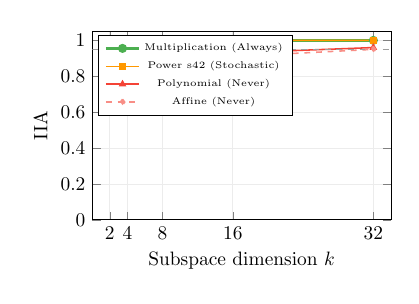
\begin{tikzpicture}[scale=0.7]
  \begin{axis}[
    width=7cm, height=5cm,
    xlabel={Subspace dimension $k$},
    ylabel={IIA},
    xmin=0, xmax=34,
    ymin=0, ymax=1.05,
    xtick={2,4,8,16,32},
    ytick={0,0.2,0.4,0.6,0.8,1.0},
    legend style={at={(0.02,0.98)},anchor=north west,font=\tiny},
    grid=major,
    grid style={neutral!20},
  ]
  % Always: multiplication — jumps to 1.0 at k=2
  \addplot[always,ultra thick,mark=*,mark size=1.5pt]
    coordinates {(2,1.0) (4,1.0) (8,1.0) (16,1.0) (32,1.0)};
  \addlegendentry{Multiplication (Always)}

  % Stochastic: power s42 — moderate
  \addplot[stoch,thick,mark=square*,mark size=1.5pt]
    coordinates {(2,0.98) (4,0.99) (8,1.0) (16,1.0) (32,1.0)};
  \addlegendentry{Power s42 (Stochastic)}

  % Never: polynomial — gradual rise
  \addplot[never,thick,mark=triangle*,mark size=1.5pt]
    coordinates {(2,0.72) (4,0.78) (8,0.88) (16,0.93) (32,0.96)};
  \addlegendentry{Polynomial (Never)}

  % Never: affine — very gradual
  \addplot[never!60,thick,dashed,mark=diamond*,mark size=1.5pt]
    coordinates {(2,0.78) (4,0.82) (8,0.87) (16,0.91) (32,0.95)};
  \addlegendentry{Affine (Never)}

  % Threshold line
  \addplot[neutral,dashed,thin] coordinates {(0,0.95) (34,0.95)};
  \end{axis}
\end{tikzpicture}
\end{column}
\begin{column}{0.48\textwidth}
\vspace{1em}
{\small \textbf{Always Grassmannian}: IIA saturates at 1.0 by $k = 2$. The causal variable is intrinsically 2-dimensional.}

\vspace{0.5em}
{\small \textbf{Never Grassmannian}: IIA rises gradually and may not reach 1.0 even at $k = 32$. More dimensions help, but the fit is never clean.}

\vspace{0.5em}
{\small The $k$-sweep profile is a \textbf{diagnostic}: if IIA keeps rising past $k = 4$, the causal variable is probably not Grassmannian.}
\end{column}
\end{columns}
\end{frame}

\section{6. Stochastic grokking}

%% --- SLIDE: Stochastic grokking ---
\begin{frame}{Stochastic grokking: same operation, opposite outcomes}

\begin{columns}[T]
\begin{column}{0.55\textwidth}
{\small The stochastic class is the strongest evidence for our claim.}

\vspace{0.3em}
{\small \textbf{Power} ($a^b \bmod 113$):}
\begin{itemize}
  \item {\small Seed 137: grokked. Equiv = 96.5\%}
  \item {\small Seed 42: not grokked. Equiv = 66.5\%}
\end{itemize}

\vspace{0.3em}
{\small \textbf{Composite addition} ($(a+b) \bmod 91$):}
\begin{itemize}
  \item {\small Original seed: grokked. Equiv = 99.8\%}
  \item {\small Seed 42: not grokked. Equiv = 11.0\%}
\end{itemize}

\vspace{0.3em}
{\small Same operation. Same architecture. Same hyperparameters. \textbf{Opposite outcomes from random initialization alone.}}

\vspace{0.3em}
\fcolorbox{grass}{grass!10}{\parbox{0.9\linewidth}{\centering\vspace{0.2em}
  {\small Grassmannian variables appear if and only if the model generalizes.}
\vspace{0.2em}}}
\end{column}
\begin{column}{0.42\textwidth}
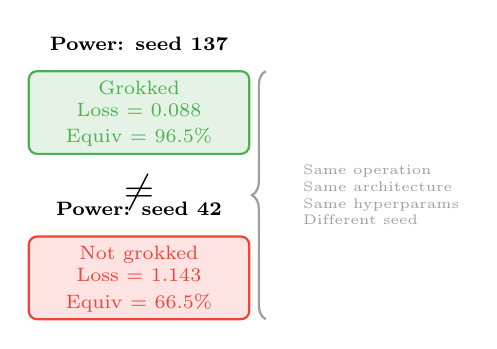
\begin{tikzpicture}[scale=0.7]
  % Seed 137
  \node[font=\scriptsize\bfseries] at (0,5.5) {Power: seed 137};
  \draw[always,thick,fill=always!15,rounded corners=3pt] (-2,3.5) rectangle (2,5.0);
  \node[font=\scriptsize,always,align=center] at (0,4.5) {Grokked\\Loss = 0.088};
  \node[font=\scriptsize,always] at (0,3.8) {Equiv = 96.5\%};

  % Seed 42
  \node[font=\scriptsize\bfseries] at (0,2.5) {Power: seed 42};
  \draw[never,thick,fill=never!15,rounded corners=3pt] (-2,0.5) rectangle (2,2.0);
  \node[font=\scriptsize,never,align=center] at (0,1.5) {Not grokked\\Loss = 1.143};
  \node[font=\scriptsize,never] at (0,0.8) {Equiv = 66.5\%};

  % Equals sign between
  \node[font=\Large] at (0,2.8) {$\neq$};

  % Same everything
  \draw[neutral,thick,decorate,decoration={brace,amplitude=5pt}] (2.3,0.5) -- (2.3,5.0);
  \node[font=\tiny,neutral,align=left,anchor=west] at (2.8,2.75) {Same operation\\Same architecture\\Same hyperparams\\Different seed};
\end{tikzpicture}
\end{column}
\end{columns}
\end{frame}

%% --- SLIDE: Equivariance testing ---
\begin{frame}{Equivariance: the geometric diagnostic}

\begin{columns}[T]
\begin{column}{0.55\textwidth}
{\small For operations with a group action, the DAS subspace should respect the algebraic symmetry.}

\vspace{0.3em}
{\small \textbf{Test}: shift input $a \to a + 1 \bmod p$. Does the DAS projection rotate by $2\pi / p$?}

\vspace{0.3em}
{\small Random subspaces: equivariance $< 1\%$.\\Always Grassmannian: equivariance $> 95\%$.\\Never Grassmannian: equivariance $< 52\%$.}

\vspace{0.5em}
{\small Equivariance distinguishes:}
\begin{itemize}
  \item {\small Genuine structure from memorization}
  \item {\small Causal variables from distributional artifacts}
  \item {\small What IIA alone cannot tell apart}
\end{itemize}
\end{column}
\begin{column}{0.42\textwidth}
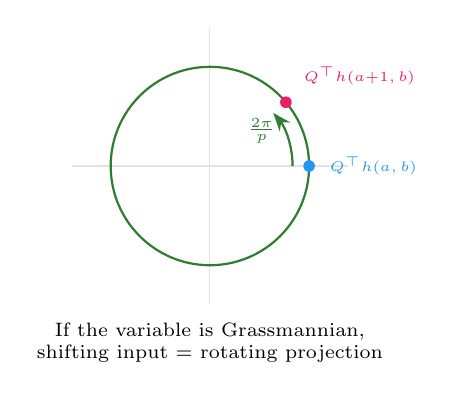
\begin{tikzpicture}[scale=0.7]
  \draw[neutral!30] (-2.5,0) -- (2.5,0);
  \draw[neutral!30] (0,-2.5) -- (0,2.5);

  % Circle
  \draw[grass,thick] (0,0) circle (1.8);

  % Point at angle 0
  \fill[das] ({1.8*cos(0)},{1.8*sin(0)}) circle (3pt);
  \node[font=\tiny,das,right] at ({2.0*cos(0)},{2.0*sin(0)}) {$Q^\top h(a,b)$};

  % Point at shifted angle
  \fill[circle] ({1.8*cos(40)},{1.8*sin(40)}) circle (3pt);
  \node[font=\tiny,circle,above right] at ({2.0*cos(40)},{2.0*sin(40)}) {$Q^\top h(a{+}1,b)$};

  % Rotation arrow
  \draw[grass,thick,-{Stealth}] ({1.5*cos(0)},{1.5*sin(0)})
    arc[start angle=0, end angle=40, radius=1.5];
  \node[font=\tiny,grass] at ({1.0*cos(20)},{1.0*sin(20)+0.3}) {$\frac{2\pi}{p}$};

  % Label
  \node[font=\scriptsize,align=center] at (0,-3.2) {If the variable is Grassmannian,\\shifting input = rotating projection};
\end{tikzpicture}
\end{column}
\end{columns}
\end{frame}


%% ============================================================
%% PART 3: THE VACUITY PROBLEM
%% ============================================================

\begin{frame}[plain]
\vfill
\begin{center}
  \setlength{\fboxrule}{2.5pt}%
  \fcolorbox{black}{white}{\parbox{0.7\textwidth}{\centering\vspace{0.8em}
    {\Large\bfseries Part 3}\\[0.5em]
    {\large The vacuity problem: when high IIA means nothing}
  \vspace{0.8em}}}
\end{center}
\vfill
\end{frame}

\section{7. Memorization artifacts}

%% --- SLIDE: Memorization produces high IIA ---
\begin{frame}{Memorization produces high IIA}

\begin{columns}[T]
\begin{column}{0.55\textwidth}
{\small Squaring ($a^2 \bmod 113$) achieves $\IIA = 0.86$ at $k = 2$ and $\IIA = 1.0$ by $k = 4$.}

\vspace{0.3em}
{\small But the model \textbf{never grokked} (test loss = 7.8). It memorized the training set.}

\vspace{0.3em}
{\small Equivariance exposes the artifact:}
\begin{itemize}
  \item {\small Squaring: 31.4\% (vs.\ $>95\%$ for genuine)}
  \item {\small Cubing: 50.9\%}
  \item {\small Random subspace: $<1\%$}
\end{itemize}

\vspace{0.5em}
\fcolorbox{fail}{fail!10}{\parbox{0.9\linewidth}{\centering\vspace{0.2em}
  {\small High IIA with low-$k$ saturation is compatible with a \textbf{lookup table}. IIA alone cannot tell the difference.}
\vspace{0.2em}}}
\end{column}
\begin{column}{0.42\textwidth}
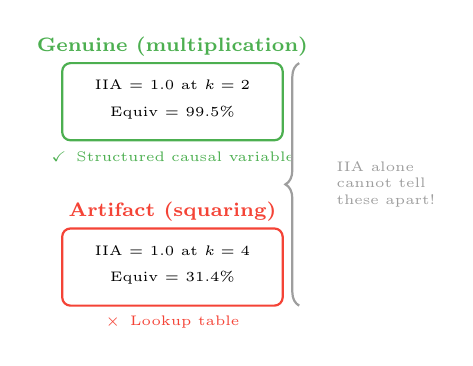
\begin{tikzpicture}[scale=0.7]
  % Genuine causal variable
  \node[font=\scriptsize\bfseries,always] at (0,5.5) {Genuine (multiplication)};
  \draw[always,thick,rounded corners=3pt] (-2,3.8) rectangle (2,5.2);
  \node[font=\tiny,align=center] at (0,4.8) {IIA = 1.0 at $k=2$};
  \node[font=\tiny,align=center] at (0,4.3) {Equiv = 99.5\%};
  \node[font=\tiny,always] at (0,3.5) {\checkmark\, Structured causal variable};

  % Memorized artifact
  \node[font=\scriptsize\bfseries,never] at (0,2.5) {Artifact (squaring)};
  \draw[never,thick,rounded corners=3pt] (-2,0.8) rectangle (2,2.2);
  \node[font=\tiny,align=center] at (0,1.8) {IIA = 1.0 at $k=4$};
  \node[font=\tiny,align=center] at (0,1.3) {Equiv = 31.4\%};
  \node[font=\tiny,never] at (0,0.5) {$\times$\, Lookup table};

  % The problem
  \draw[neutral,thick,decorate,decoration={brace,amplitude=5pt}] (2.3,0.8) -- (2.3,5.2);
  \node[font=\tiny,neutral,align=left,anchor=west] at (2.8,3.0) {IIA alone\\cannot tell\\these apart!};
\end{tikzpicture}
\end{column}
\end{columns}
\end{frame}

\section{8. NL-DAS is vacuous}

%% --- SLIDE: The NL-DAS idea ---
\begin{frame}{The natural response: add nonlinearity}

\begin{columns}[T]
\begin{column}{0.55\textwidth}
{\small DAS assumes linearity and fails on nonlinear variables. Natural fix: prepend an MLP featurizer.}

\vspace{0.3em}
{\small \textbf{NL-DAS}: learn encoder $f$ and decoder $g$, then apply linear DAS in the transformed space:}

$$h' = g\bigl(f(h_b) - QQ^\top f(h_b) + QQ^\top f(h_s)\bigr)$$

\vspace{0.3em}
{\small Result on IOI (GPT-2):}
\begin{itemize}
  \item {\small DAS at $k=1$: IIA = 0.193}
  \item {\small NL-DAS at $k=1$: IIA = \textbf{1.000}}
\end{itemize}

\vspace{0.3em}
{\small This looks like a dramatic improvement.}

\vspace{0.3em}
{\Large \textbf{It is not.}}
\end{column}
\begin{column}{0.42\textwidth}
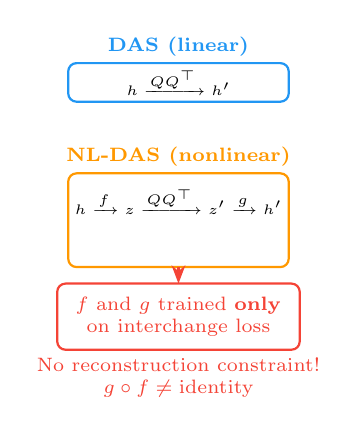
\begin{tikzpicture}[scale=0.7]
  % DAS path
  \node[font=\scriptsize\bfseries,das] at (0,5.5) {DAS (linear)};
  \draw[das,thick,rounded corners=3pt] (-2,4.5) rectangle (2,5.2);
  \node[font=\tiny] at (0,4.85) {$h \xrightarrow{QQ^\top} h'$};

  % NL-DAS path
  \node[font=\scriptsize\bfseries,nldas] at (0,3.5) {NL-DAS (nonlinear)};
  \draw[nldas,thick,rounded corners=3pt] (-2,1.5) rectangle (2,3.2);
  \node[font=\tiny,align=center] at (0,2.7) {$h \xrightarrow{f} z \xrightarrow{QQ^\top} z' \xrightarrow{g} h'$};

  % The problem
  \draw[fail,thick,rounded corners=3pt] (-2.2,0.0) rectangle (2.2,1.2);
  \node[font=\scriptsize,fail,align=center] at (0,0.6) {$f$ and $g$ trained \textbf{only}\\on interchange loss};

  % Arrow
  \draw[fail,thick,-{Stealth}] (0,1.5) -- (0,1.2);

  \node[font=\scriptsize,fail,align=center] at (0,-0.5) {No reconstruction constraint!\\$g \circ f \neq \text{identity}$};
\end{tikzpicture}
\end{column}
\end{columns}
\end{frame}

%% --- SLIDE: The lookup table failure ---
\begin{frame}{The lookup-table failure mode}

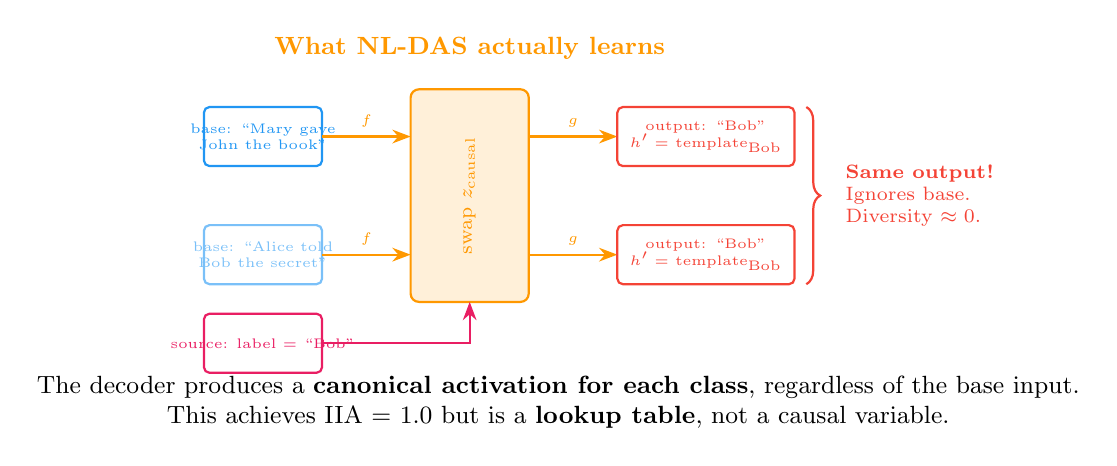
\begin{tikzpicture}[scale=0.75]
  % Left: what NL-DAS actually does
  \node[font=\small\bfseries,nldas] at (0,4.5) {What NL-DAS actually learns};

  % Different base inputs
  \draw[das,thick,rounded corners=2pt] (-4.5,2.5) rectangle (-2.5,3.5);
  \node[font=\tiny,das,align=center] at (-3.5,3.0) {base: ``Mary gave\\John the book''};

  \draw[das!60,thick,rounded corners=2pt] (-4.5,0.5) rectangle (-2.5,1.5);
  \node[font=\tiny,das!60,align=center] at (-3.5,1.0) {base: ``Alice told\\Bob the secret''};

  % Encoder
  \draw[nldas,thick,-{Stealth}] (-2.5,3.0) -- (-1,3.0);
  \draw[nldas,thick,-{Stealth}] (-2.5,1.0) -- (-1,1.0);
  \node[font=\tiny,nldas,above] at (-1.75,3.0) {$f$};
  \node[font=\tiny,nldas,above] at (-1.75,1.0) {$f$};

  % Swap box
  \fill[nldas!15,rounded corners=3pt] (-1,0.2) rectangle (1,3.8);
  \draw[nldas,thick,rounded corners=3pt] (-1,0.2) rectangle (1,3.8);
  \node[font=\scriptsize,nldas,rotate=90] at (0,2.0) {swap $z_\text{causal}$};

  % Same source
  \draw[circle,thick,rounded corners=2pt] (-4.5,-1.0) rectangle (-2.5,0.0);
  \node[font=\tiny,circle,align=center] at (-3.5,-0.5) {source: label = ``Bob''};
  \draw[circle,thick,-{Stealth}] (-2.5,-0.5) -- (0,-0.5) -- (0,0.2);

  % Decoder
  \draw[nldas,thick,-{Stealth}] (1,3.0) -- (2.5,3.0);
  \draw[nldas,thick,-{Stealth}] (1,1.0) -- (2.5,1.0);
  \node[font=\tiny,nldas,above] at (1.75,3.0) {$g$};
  \node[font=\tiny,nldas,above] at (1.75,1.0) {$g$};

  % Outputs — SAME
  \draw[fail,thick,rounded corners=2pt] (2.5,2.5) rectangle (5.5,3.5);
  \node[font=\tiny,fail,align=center] at (4.0,3.0) {output: ``Bob''\\$h' = $ template$_\text{Bob}$};

  \draw[fail,thick,rounded corners=2pt] (2.5,0.5) rectangle (5.5,1.5);
  \node[font=\tiny,fail,align=center] at (4.0,1.0) {output: ``Bob''\\$h' = $ template$_\text{Bob}$};

  % Same!
  \draw[fail,thick,decorate,decoration={brace,amplitude=5pt,mirror}] (5.7,0.5) -- (5.7,3.5);
  \node[font=\scriptsize,fail,align=left,anchor=west] at (6.2,2.0) {\textbf{Same output!}\\Ignores base.\\Diversity $\approx 0$.};

  % Bottom
  \node[font=\small,align=center] at (1.5,-1.5) {The decoder produces a \textbf{canonical activation for each class}, regardless of the base input.\\This achieves IIA = 1.0 but is a \textbf{lookup table}, not a causal variable.};
\end{tikzpicture}
\end{frame}

%% --- SLIDE: NL-DAS table ---
\begin{frame}{NL-DAS vs.\ DAS vs.\ structured VAE}

\centering
{\small\setlength{\tabcolsep}{4pt}
\begin{tabular}{lc rrrr}
\toprule
\textbf{Task} & $\boldsymbol{k}$ & \textbf{DAS} & \textbf{NL-DAS} & \textbf{VAE} & \textbf{Assessment} \\
\midrule
IOI & 1 & 0.193 & \textcolor{fail}{\textbf{1.000}} & 0.232 & NL-DAS vacuous \\
IOI & 2 & 0.297 & \textcolor{fail}{\textbf{1.000}} & 0.719 & NL-DAS vacuous \\
IOI & 4 & 0.556 & \textcolor{fail}{\textbf{1.000}} & \textcolor{pass}{\textbf{0.978}} & VAE genuine \\
Addition & 1 & 0.006 & 0.194 & 0.000 & Both honest \\
Addition & 4 & 0.289 & \textcolor{fail}{\textbf{0.883}} & 0.089 & NL-DAS suspect \\
Mult. & 4 & 0.344 & \textcolor{fail}{\textbf{0.961}} & 0.000 & NL-DAS suspect \\
Squaring & $*$ & 0.000 & 0.011 & 0.000 & No structure \\
\bottomrule
\end{tabular}}

\vspace{0.5em}
{\small \textcolor{fail}{Red bold}: suspiciously high IIA. \textcolor{pass}{Green bold}: validated by diversity ratio.}

\vspace{0.3em}
{\small NL-DAS achieves IIA $\approx 1$ on IOI at $k=1$ --- that is getting perfect interchange accuracy from a \textbf{single dimension}. Diversity ratio $\approx 0$ confirms it is a lookup table.}
\end{frame}

\section{9. Intervention faithfulness}

%% --- SLIDE: Diversity ratio ---
\begin{frame}{The diversity ratio: detecting lookup tables}

\begin{columns}[T]
\begin{column}{0.55\textwidth}
{\small For each source label $y_s$, compute the standard deviation of intervened activations $h'$ across all base inputs:}

$$\rho = \frac{\mathbb{E}_{y_s}\bigl[\text{std}(h'_{y_s})\bigr]}{\mathbb{E}_{y_s}\bigl[\text{std}(h_{y_s})\bigr]}$$

\vspace{0.3em}
{\small $\rho \approx 0$: all intervened activations for the same source label collapse to a single point. \textbf{Lookup table.}}

\vspace{0.3em}
{\small $\rho \approx 1$: the intervention preserves natural variation within each class. \textbf{Genuine intervention.}}

\vspace{0.3em}
{\small This is the key metric that exposes NL-DAS: it achieves IIA = 1.0 but $\rho \approx 0$.}
\end{column}
\begin{column}{0.42\textwidth}
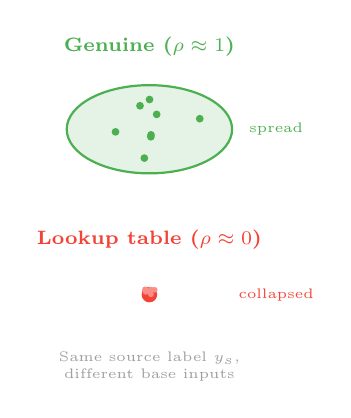
\begin{tikzpicture}[scale=0.7]
  % Genuine intervention
  \node[font=\scriptsize\bfseries,pass] at (0,5.5) {Genuine ($\rho \approx 1$)};
  \fill[pass!15] (0,4.0) ellipse (1.5 and 0.8);
  \draw[pass,thick] (0,4.0) ellipse (1.5 and 0.8);
  \foreach \i in {1,...,8} {
    \pgfmathsetmacro{\x}{1.2*rand}
    \pgfmathsetmacro{\y}{0.6*rand}
    \fill[pass] (\x,4.0+\y) circle (2pt);
  }
  \node[font=\tiny,pass] at (2.3,4.0) {spread};

  % Lookup table
  \node[font=\scriptsize\bfseries,fail] at (0,2.0) {Lookup table ($\rho \approx 0$)};
  \fill[fail] (0,1.0) circle (4pt);
  \foreach \i in {1,...,8} {
    \pgfmathsetmacro{\x}{0.1*rand}
    \pgfmathsetmacro{\y}{0.1*rand}
    \fill[fail!60] (\x,1.0+\y) circle (1.5pt);
  }
  \node[font=\tiny,fail] at (2.3,1.0) {collapsed};

  % Label
  \node[font=\tiny,neutral,align=center] at (0,-0.3) {Same source label $y_s$,\\different base inputs};
\end{tikzpicture}
\end{column}
\end{columns}
\end{frame}

%% --- SLIDE: Four faithfulness metrics ---
\begin{frame}{Four complementary faithfulness metrics}

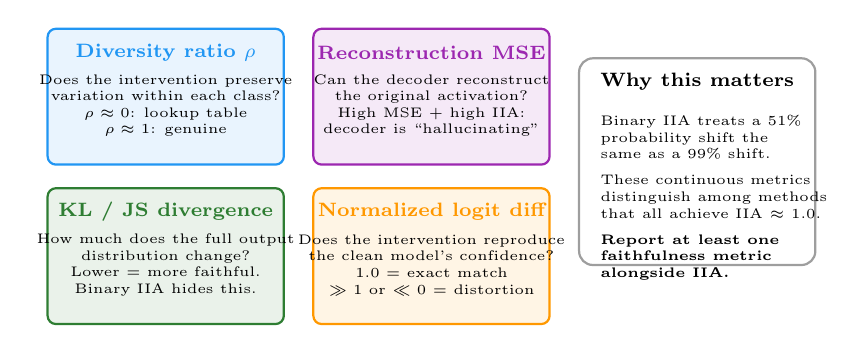
\begin{tikzpicture}[scale=0.75]
  % Metric 1: Diversity ratio
  \fill[das!10,rounded corners=3pt] (-5.5,2.2) rectangle (-1.5,4.5);
  \draw[das,thick,rounded corners=3pt] (-5.5,2.2) rectangle (-1.5,4.5);
  \node[font=\scriptsize\bfseries,das] at (-3.5,4.1) {Diversity ratio $\rho$};
  \node[font=\tiny,align=center] at (-3.5,3.2) {Does the intervention preserve\\variation within each class?\\$\rho \approx 0$: lookup table\\$\rho \approx 1$: genuine};

  % Metric 2: Reconstruction fidelity
  \fill[vae!10,rounded corners=3pt] (-1,2.2) rectangle (3,4.5);
  \draw[vae,thick,rounded corners=3pt] (-1,2.2) rectangle (3,4.5);
  \node[font=\scriptsize\bfseries,vae] at (1,4.1) {Reconstruction MSE};
  \node[font=\tiny,align=center] at (1,3.2) {Can the decoder reconstruct\\the original activation?\\High MSE + high IIA:\\decoder is ``hallucinating''};

  % Metric 3: KL / JS divergence
  \fill[grass!10,rounded corners=3pt] (-5.5,-0.5) rectangle (-1.5,1.8);
  \draw[grass,thick,rounded corners=3pt] (-5.5,-0.5) rectangle (-1.5,1.8);
  \node[font=\scriptsize\bfseries,grass] at (-3.5,1.4) {KL / JS divergence};
  \node[font=\tiny,align=center] at (-3.5,0.5) {How much does the full output\\distribution change?\\Lower = more faithful.\\Binary IIA hides this.};

  % Metric 4: Normalized logit diff
  \fill[nldas!10,rounded corners=3pt] (-1,-0.5) rectangle (3,1.8);
  \draw[nldas,thick,rounded corners=3pt] (-1,-0.5) rectangle (3,1.8);
  \node[font=\scriptsize\bfseries,nldas] at (1,1.4) {Normalized logit diff};
  \node[font=\tiny,align=center] at (1,0.5) {Does the intervention reproduce\\the clean model's confidence?\\1.0 = exact match\\$\gg 1$ or $\ll 0$ = distortion};

  % Why this matters
  \draw[neutral,thick,rounded corners=5pt] (3.5,0.5) rectangle (7.5,4.0);
  \node[font=\scriptsize\bfseries] at (5.5,3.6) {Why this matters};
  \node[font=\tiny,align=left,anchor=north west] at (3.7,3.2) {%
    Binary IIA treats a 51\%\\
    probability shift the\\
    same as a 99\% shift.\\[0.5em]
    These continuous metrics\\
    distinguish among methods\\
    that all achieve IIA $\approx$ 1.0.\\[0.5em]
    \textbf{Report at least one}\\
    \textbf{faithfulness metric}\\
    \textbf{alongside IIA.}};
\end{tikzpicture}
\end{frame}


%% ============================================================
%% PART 4: THE FIX
%% ============================================================

\begin{frame}[plain]
\vfill
\begin{center}
  \setlength{\fboxrule}{2.5pt}%
  \fcolorbox{black}{white}{\parbox{0.7\textwidth}{\centering\vspace{0.8em}
    {\Large\bfseries Part 4}\\[0.5em]
    {\large The fix: structured VAE and cross-task transfer}
  \vspace{0.8em}}}
\end{center}
\vfill
\end{frame}

\section{10. Structured VAE}

%% --- SLIDE: The structured VAE idea ---
\begin{frame}{Structured VAE for nonlinear causal variables}

\begin{columns}[T]
\begin{column}{0.55\textwidth}
{\small The structured VAE partitions the latent space into:}
\begin{itemize}
  \item {\small $z_\text{causal}$: supervised with the operation's label}
  \item {\small $z_\text{nuisance}$: unsupervised, absorbs everything else}
\end{itemize}

\vspace{0.3em}
{\small The loss combines three terms:}
$$\mathcal{L} = \underbrace{-\mathbb{E}_q[\log p(x \mid y, z)]}_{\text{reconstruction}} + \beta \underbrace{D_\text{KL}}_{\text{regularization}} + \alpha \underbrace{\mathcal{L}_\text{CE}}_{\text{supervision}}$$

\vspace{0.3em}
{\small The ELBO prevents the lookup-table failure:}
\begin{enumerate}
  \item {\small Reconstruction forces faithful decoding}
  \item {\small KL prevents latent collapse}
  \item {\small Causal/nuisance split preserves base info}
\end{enumerate}
\end{column}
\begin{column}{0.42\textwidth}
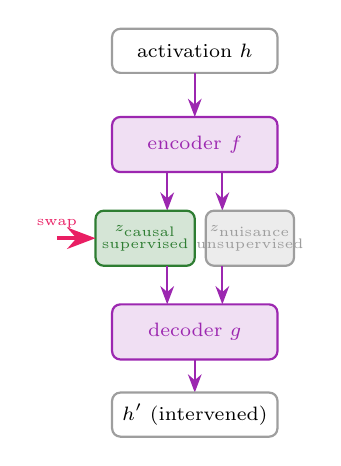
\begin{tikzpicture}[scale=0.7]
  % Input
  \draw[neutral,thick,rounded corners=3pt] (-1.5,5.0) rectangle (1.5,5.8);
  \node[font=\scriptsize] at (0,5.4) {activation $h$};

  % Encoder
  \draw[vae,thick,-{Stealth}] (0,5.0) -- (0,4.2);
  \draw[vae,thick,rounded corners=3pt,fill=vae!15] (-1.5,3.2) rectangle (1.5,4.2);
  \node[font=\scriptsize,vae] at (0,3.7) {encoder $f$};

  % Split
  \draw[vae,thick,-{Stealth}] (-0.5,3.2) -- (-0.5,2.5);
  \draw[vae,thick,-{Stealth}] (0.5,3.2) -- (0.5,2.5);

  % Causal latent
  \fill[grass!20,rounded corners=3pt] (-1.8,1.5) rectangle (0,2.5);
  \draw[grass,thick,rounded corners=3pt] (-1.8,1.5) rectangle (0,2.5);
  \node[font=\tiny,grass,align=center] at (-0.9,2.0) {$z_\text{causal}$\\{\tiny supervised}};

  % Nuisance latent
  \fill[neutral!20,rounded corners=3pt] (0.2,1.5) rectangle (1.8,2.5);
  \draw[neutral,thick,rounded corners=3pt] (0.2,1.5) rectangle (1.8,2.5);
  \node[font=\tiny,neutral,align=center] at (1.0,2.0) {$z_\text{nuisance}$\\{\tiny unsupervised}};

  % Swap arrow
  \draw[circle,ultra thick,-{Stealth}] (-2.5,2.0) -- (-1.8,2.0);
  \node[font=\tiny,circle,above] at (-2.5,2.0) {swap};

  % Decoder
  \draw[vae,thick,-{Stealth}] (-0.5,1.5) -- (-0.5,0.8);
  \draw[vae,thick,-{Stealth}] (0.5,1.5) -- (0.5,0.8);
  \draw[vae,thick,rounded corners=3pt,fill=vae!15] (-1.5,-0.2) rectangle (1.5,0.8);
  \node[font=\scriptsize,vae] at (0,0.3) {decoder $g$};

  % Output
  \draw[vae,thick,-{Stealth}] (0,-0.2) -- (0,-0.8);
  \draw[neutral,thick,rounded corners=3pt] (-1.5,-1.6) rectangle (1.5,-0.8);
  \node[font=\scriptsize] at (0,-1.2) {$h'$ (intervened)};
\end{tikzpicture}
\end{column}
\end{columns}
\end{frame}

%% --- SLIDE: Why VAE is not vacuous ---
\begin{frame}{Why the VAE is not vacuous: three constraints}

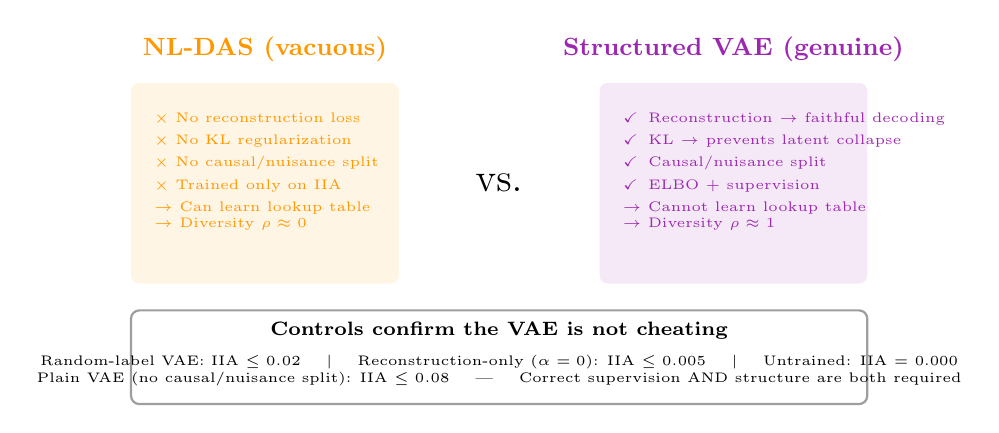
\begin{tikzpicture}[scale=0.85]
  % NL-DAS column
  \node[font=\small\bfseries,nldas] at (-3.5,4.5) {NL-DAS (vacuous)};

  \fill[nldas!10,rounded corners=3pt] (-5.5,1.0) rectangle (-1.5,4.0);
  \node[font=\tiny,nldas,align=left,anchor=north west] at (-5.3,3.7) {%
    $\times$ No reconstruction loss\\[0.3em]
    $\times$ No KL regularization\\[0.3em]
    $\times$ No causal/nuisance split\\[0.3em]
    $\times$ Trained only on IIA\\[0.3em]
    $\to$ Can learn lookup table\\
    $\to$ Diversity $\rho \approx 0$};

  % Arrow
  \node[font=\Large] at (0,2.5) {vs.};

  % VAE column
  \node[font=\small\bfseries,vae] at (3.5,4.5) {Structured VAE (genuine)};

  \fill[vae!10,rounded corners=3pt] (1.5,1.0) rectangle (5.5,4.0);
  \node[font=\tiny,vae,align=left,anchor=north west] at (1.7,3.7) {%
    \checkmark\, Reconstruction $\to$ faithful decoding\\[0.3em]
    \checkmark\, KL $\to$ prevents latent collapse\\[0.3em]
    \checkmark\, Causal/nuisance split\\[0.3em]
    \checkmark\, ELBO + supervision\\[0.3em]
    $\to$ Cannot learn lookup table\\
    $\to$ Diversity $\rho \approx 1$};

  % Controls
  \draw[neutral,thick,rounded corners=3pt] (-5.5,-0.8) rectangle (5.5,0.6);
  \node[font=\scriptsize\bfseries] at (0,0.3) {Controls confirm the VAE is not cheating};
  \node[font=\tiny,align=center] at (0,-0.3) {Random-label VAE: IIA $\leq 0.02$ \quad $|$ \quad Reconstruction-only ($\alpha = 0$): IIA $\leq 0.005$ \quad $|$ \quad Untrained: IIA = 0.000\\
  Plain VAE (no causal/nuisance split): IIA $\leq 0.08$ \quad --- \quad Correct supervision AND structure are both required};
\end{tikzpicture}
\end{frame}

%% --- SLIDE: VAE matches DAS where DAS works ---
\begin{frame}{VAE matches DAS where DAS works, extends where it fails}

\begin{columns}[T]
\begin{column}{0.48\textwidth}
{\small \textbf{Always Grassmannian operations:}\\VAE reduces to an effective rotation.}

\vspace{0.3em}
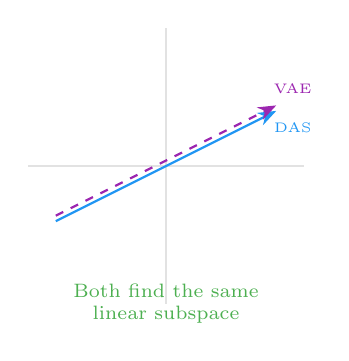
\begin{tikzpicture}[scale=0.7]
  % DAS and VAE agree
  \draw[neutral!30] (-2.5,0) -- (2.5,0);
  \draw[neutral!30] (0,-2.5) -- (0,2.5);

  % Linear subspace
  \draw[das,thick,-{Stealth}] (-2,-1) -- (2,1);
  \draw[vae,thick,dashed,-{Stealth}] (-2,-0.9) -- (2,1.1);

  \node[font=\tiny,das] at (2.3,0.7) {DAS};
  \node[font=\tiny,vae] at (2.3,1.4) {VAE};

  \node[font=\scriptsize,pass,align=center] at (0,-2.5) {Both find the same\\linear subspace};
\end{tikzpicture}
\end{column}
\begin{column}{0.48\textwidth}
{\small \textbf{Never Grassmannian operations:}\\VAE's nonlinear encoder captures curved structure.}

\vspace{0.3em}
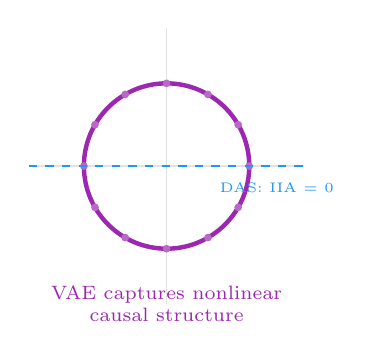
\begin{tikzpicture}[scale=0.7]
  \draw[neutral!30] (-2.5,0) -- (2.5,0);
  \draw[neutral!30] (0,-2.5) -- (0,2.5);

  % Circle
  \draw[vae,ultra thick] (0,0) circle (1.5);
  \foreach \a in {0,30,...,330} {
    \fill[vae!70] ({1.5*cos(\a)},{1.5*sin(\a)}) circle (2pt);
  }

  % DAS fails
  \draw[das,thick,dashed] (-2.5,0) -- (2.5,0);
  \node[font=\tiny,das] at (2.0,-0.4) {DAS: IIA = 0};

  \node[font=\scriptsize,vae,align=center] at (0,-2.5) {VAE captures nonlinear\\causal structure};
\end{tikzpicture}
\end{column}
\end{columns}

\vspace{0.5em}
\centering
{\small For grokked addition and multiplication, both DAS and VAE achieve IIA = 1.000 and equivariance $>99\%$.\\The VAE is a \textbf{strict generalization} of DAS: when the variable is linear, VAE = DAS.}
\end{frame}

\section{11. Cross-task transfer}

%% --- SLIDE: Cross-task transfer on IOI ---
\begin{frame}{Cross-task transfer validates causal variables}

\begin{columns}[T]
\begin{column}{0.55\textwidth}
{\small A genuine causal variable should \textbf{transfer} --- train on one task variant, test on another.}

\vspace{0.3em}
{\small \textbf{IOI cross-template transfer} (GPT-2):}
\begin{itemize}
  \item {\small Train VAE on templates 1--3}
  \item {\small Test on unseen templates 4--5}
  \item {\small IIA = 0.82--0.96 at $k = 4$}
\end{itemize}

\vspace{0.3em}
{\small \textbf{Jensen's extended IOI tasks}:}
\begin{itemize}
  \item {\small DoubleIO: IIA = 0.77--0.81}
  \item {\small TripleIO: IIA = 0.77--0.81}
  \item {\small Trained only on base IOI!}
\end{itemize}

\vspace{0.3em}
{\small \textbf{IOI subtask transfer} (8 MIB counterfactual types):}
\begin{itemize}
  \item {\small DAS transfer ratio: 0.56}
  \item {\small VAE transfer ratio: 0.43}
\end{itemize}
\end{column}
\begin{column}{0.42\textwidth}
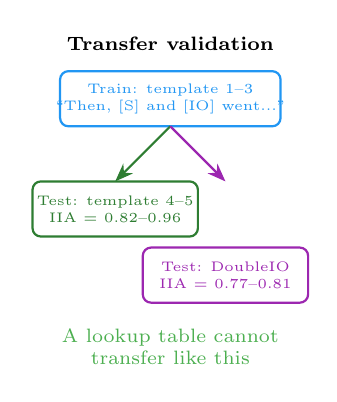
\begin{tikzpicture}[scale=0.7]
  % Transfer diagram
  \node[font=\scriptsize\bfseries] at (0,5.0) {Transfer validation};

  % Train
  \draw[das,thick,rounded corners=3pt] (-2,3.5) rectangle (2,4.5);
  \node[font=\tiny,das,align=center] at (0,4.0) {Train: template 1--3\\``Then, [S] and [IO] went...''};

  % Test 1
  \draw[grass,thick,-{Stealth}] (0,3.5) -- (-1,2.5);
  \draw[grass,thick,rounded corners=3pt] (-2.5,1.5) rectangle (0.5,2.5);
  \node[font=\tiny,grass,align=center] at (-1,2.0) {Test: template 4--5\\IIA = 0.82--0.96};

  % Test 2
  \draw[vae,thick,-{Stealth}] (0,3.5) -- (1,2.5);
  \draw[vae,thick,rounded corners=3pt] (-0.5,0.3) rectangle (2.5,1.3);
  \node[font=\tiny,vae,align=center] at (1,0.8) {Test: DoubleIO\\IIA = 0.77--0.81};

  % The point
  \node[font=\scriptsize,pass,align=center] at (0,-0.5) {A lookup table cannot\\transfer like this};
\end{tikzpicture}
\end{column}
\end{columns}
\end{frame}

\section{12. IOI is not Grassmannian}

%% --- SLIDE: Sheaf consistency ---
\begin{frame}{IOI is NOT Grassmannian: sheaf consistency analysis}

\begin{columns}[T]
\begin{column}{0.55\textwidth}
{\small Even within GPT-2's IOI circuit, the causal variable is not globally linear.}

\vspace{0.3em}
{\small We fit local DAS subspaces to different clusters of activations and measure consistency:}

\vspace{0.3em}
\begin{itemize}
  \item {\small Geodesic distance between local subspaces: \textbf{$\sim$2.2}}
  \item {\small Cross-cluster IIA: \textbf{$\sim$0.21}}
\end{itemize}

\vspace{0.3em}
{\small If IOI were Grassmannian, local subspaces would agree (geodesic $\approx 0$, cross-IIA $\approx 1.0$).}

\vspace{0.3em}
{\small The subspace that represents the indirect object \textbf{rotates} across different activation clusters. Locally linear, globally nonlinear --- like a curved manifold approximated by tangent planes.}

\vspace{0.3em}
{\small This is why the VAE outperforms DAS on IOI at $k = 4$ (IIA 0.978 vs.\ 0.556).}
\end{column}
\begin{column}{0.42\textwidth}
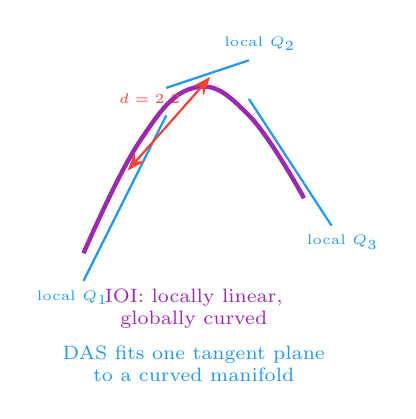
\begin{tikzpicture}[scale=0.7]
  % Curved manifold
  \draw[vae,ultra thick] plot[smooth,tension=0.7]
    coordinates {(-2,-1) (-1,1) (0,2) (1,1.5) (2,0)};

  % Local tangent planes
  \draw[das,thick] (-2.0,-1.5) -- (-0.5,1.5);
  \node[font=\tiny,das] at (-2.2,-1.8) {local $Q_1$};

  \draw[das,thick] (-0.5,2.0) -- (1.0,2.5);
  \node[font=\tiny,das] at (1.2,2.8) {local $Q_2$};

  \draw[das,thick] (1.0,1.8) -- (2.5,-0.5);
  \node[font=\tiny,das] at (2.7,-0.8) {local $Q_3$};

  % Geodesic distances
  \draw[never,thick,{Stealth}-{Stealth}] (-1.2,0.5) -- (0.3,2.2);
  \node[font=\tiny,never] at (-0.8,1.8) {$d = 2.2$};

  % Label
  \node[font=\scriptsize,vae,align=center] at (0,-2.0) {IOI: locally linear,\\globally curved};
  \node[font=\scriptsize,das,align=center] at (0,-3.0) {DAS fits one tangent plane\\to a curved manifold};
\end{tikzpicture}
\end{column}
\end{columns}
\end{frame}


%% ============================================================
%% PART 5: IMPLICATIONS
%% ============================================================

\begin{frame}[plain]
\vfill
\begin{center}
  \setlength{\fboxrule}{2.5pt}%
  \fcolorbox{black}{white}{\parbox{0.7\textwidth}{\centering\vspace{0.8em}
    {\Large\bfseries Part 5}\\[0.5em]
    {\large Implications and practical advice}
  \vspace{0.8em}}}
\end{center}
\vfill
\end{frame}

\section{13. Four-level hierarchy}

%% --- SLIDE: The hierarchy ---
\begin{frame}{A four-level hierarchy for causal validity}

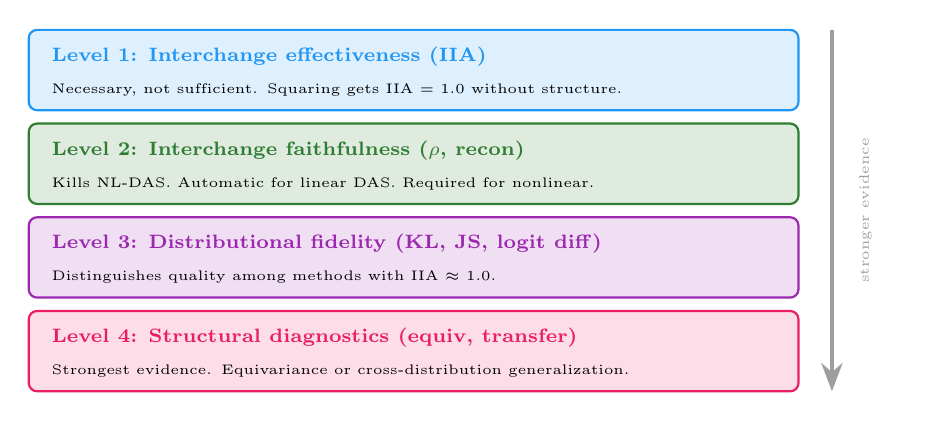
\begin{tikzpicture}[scale=0.85]
  % Level 1
  \fill[das!15,rounded corners=3pt] (-5.5,3.2) rectangle (6,4.4);
  \draw[das,thick,rounded corners=3pt] (-5.5,3.2) rectangle (6,4.4);
  \node[font=\scriptsize\bfseries,das,anchor=west] at (-5.3,4.0) {Level 1: Interchange effectiveness (IIA)};
  \node[font=\tiny,anchor=west,text width=10.8cm] at (-5.3,3.5) {Necessary, not sufficient. Squaring gets IIA = 1.0 without structure.};

  % Level 2
  \fill[grass!15,rounded corners=3pt] (-5.5,1.8) rectangle (6,3.0);
  \draw[grass,thick,rounded corners=3pt] (-5.5,1.8) rectangle (6,3.0);
  \node[font=\scriptsize\bfseries,grass,anchor=west] at (-5.3,2.6) {Level 2: Interchange faithfulness ($\rho$, recon)};
  \node[font=\tiny,anchor=west,text width=10.8cm] at (-5.3,2.1) {Kills NL-DAS. Automatic for linear DAS. Required for nonlinear.};

  % Level 3
  \fill[vae!15,rounded corners=3pt] (-5.5,0.4) rectangle (6,1.6);
  \draw[vae,thick,rounded corners=3pt] (-5.5,0.4) rectangle (6,1.6);
  \node[font=\scriptsize\bfseries,vae,anchor=west] at (-5.3,1.2) {Level 3: Distributional fidelity (KL, JS, logit diff)};
  \node[font=\tiny,anchor=west,text width=10.8cm] at (-5.3,0.7) {Distinguishes quality among methods with IIA $\approx$ 1.0.};

  % Level 4
  \fill[circle!15,rounded corners=3pt] (-5.5,-1.0) rectangle (6,0.2);
  \draw[circle,thick,rounded corners=3pt] (-5.5,-1.0) rectangle (6,0.2);
  \node[font=\scriptsize\bfseries,circle,anchor=west] at (-5.3,-0.2) {Level 4: Structural diagnostics (equiv, transfer)};
  \node[font=\tiny,anchor=west,text width=10.8cm] at (-5.3,-0.7) {Strongest evidence. Equivariance or cross-distribution generalization.};

  % Strength arrow
  \draw[neutral,ultra thick,-{Stealth}] (6.5,4.4) -- (6.5,-1.0);
  \node[font=\tiny,neutral,rotate=90] at (7.0,1.7) {stronger evidence};
\end{tikzpicture}

\vspace{0.5em}
{\small \textbf{Key asymmetry}: Linear DAS automatically passes Level 2 (orthogonal projection is faithful by construction) but may fail Level 1 on nonlinear variables. NL-DAS easily passes Level 1 but fails Level 2.}
\end{frame}

\section{14. Continuous metrics}

%% --- SLIDE: Binary vs continuous ---
\begin{frame}{Binary IIA hides important differences}

\begin{columns}[T]
\begin{column}{0.48\textwidth}
\centering
\textbf{Binary IIA}

\vspace{0.3em}
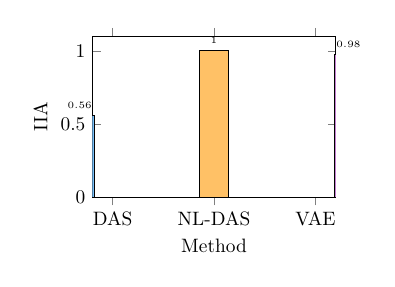
\begin{tikzpicture}[scale=0.7]
  \begin{axis}[
    width=6cm, height=4.5cm,
    ybar,
    bar width=15pt,
    xlabel={Method},
    ylabel={IIA},
    ymin=0, ymax=1.1,
    xtick={1,2,3},
    xticklabels={DAS,NL-DAS,VAE},
    ytick={0,0.5,1.0},
    nodes near coords,
    every node near coord/.append style={font=\tiny},
  ]
  \addplot[fill=das!60] coordinates {(1,0.556)};
  \addplot[fill=nldas!60] coordinates {(2,1.000)};
  \addplot[fill=vae!60] coordinates {(3,0.978)};
  \end{axis}
\end{tikzpicture}

{\small NL-DAS ``wins.'' But it is a lookup table.}
\end{column}
\begin{column}{0.48\textwidth}
\centering
\textbf{With faithfulness metrics}

\vspace{0.3em}
{\small\setlength{\tabcolsep}{2pt}
\begin{tabular}{lccc}
\toprule
& \textbf{DAS} & \textbf{NL-DAS} & \textbf{VAE} \\
\midrule
IIA & 0.556 & \textcolor{fail}{1.000} & \textcolor{pass}{0.978} \\
Diversity $\rho$ & 1.0 & \textcolor{fail}{$\approx 0$} & \textcolor{pass}{$\approx 1$} \\
Transfer & Yes & \textcolor{fail}{No} & \textcolor{pass}{Yes} \\
\bottomrule
\end{tabular}}

\vspace{0.5em}
{\small VAE wins genuinely. NL-DAS is disqualified by $\rho \approx 0$.}

\vspace{0.3em}
{\small DAS is honest but limited by linearity.}
\end{column}
\end{columns}
\end{frame}

\section{15. Practical advice}

%% --- SLIDE: Practical advice ---
\begin{frame}{Practical advice for causal abstraction}

\begin{enumerate}
  \item {\small \textbf{Never report IIA alone.} IIA = 1.0 is compatible with genuine structure, memorized lookup tables, and degenerate encoder-decoders. Always report at least one faithfulness metric.}

  \vspace{0.3em}
  \item {\small \textbf{Use continuous distributional metrics.} KL divergence and normalized logit difference distinguish among methods that all achieve IIA $\approx 1.0$. Binary IIA treats a 51\% shift the same as 99\%.}

  \vspace{0.3em}
  \item {\small \textbf{Be suspicious of unconstrained nonlinear featurizers.} Any encoder-decoder trained end-to-end on interchange loss without reconstruction constraints can learn a lookup table. The ELBO (or equivalent) is necessary.}

  \vspace{0.3em}
  \item {\small \textbf{Test cross-distribution generalization.} Evaluate on disjoint names, novel templates, or new task variants. A method that fails under distribution shift is exploiting surface regularities.}

  \vspace{0.3em}
  \item {\small \textbf{Consider nonlinear methods when DAS IIA is low.} Low IIA does not mean no causal variable --- it may mean DAS is searching the wrong function class. But validate with faithfulness metrics.}
\end{enumerate}
\end{frame}

%% --- SLIDE: Surprising cases ---
\begin{frame}{Surprising positive and negative cases}

\begin{columns}[T]
\begin{column}{0.48\textwidth}
\textbf{\textcolor{pass}{Surprising positives}}

\vspace{0.3em}
{\small \textbf{Cubic sum} ($a^3 + b^3$): perfect equivariance (100\%) despite cubing alone reaching only 50.9\%. The boundary is not ``group action vs.\ polynomial'' but whether the binary structure provides sufficient additive symmetry.}

\vspace{0.5em}
{\small \textbf{Max} ($\max(a,b)$): achieves 95.7\% equivariance despite not being a group action. It is piecewise equivariant: when the argmax is stable under shift, max behaves like a shifted identity.}
\end{column}
\begin{column}{0.48\textwidth}
\textbf{\textcolor{fail}{Surprising negatives}}

\vspace{0.3em}
{\small \textbf{Affine} ($2a + 3b + 5$): a \emph{linear} function that \emph{fails} to produce a Grassmannian variable! Under $a \mapsto a + g$, the output shifts by $2g$, not $g$. Equivariance requires the operation to be a group action, not merely linear.}

\vspace{0.5em}
{\small \textbf{Squaring}: achieves IIA = 1.0 by $k = 4$ without grokking. High IIA is the illusion; low equivariance (31.4\%) is the truth.}
\end{column}
\end{columns}
\end{frame}

\section{16. Conclusion}

%% --- SLIDE: Summary ---
\begin{frame}{Summary}

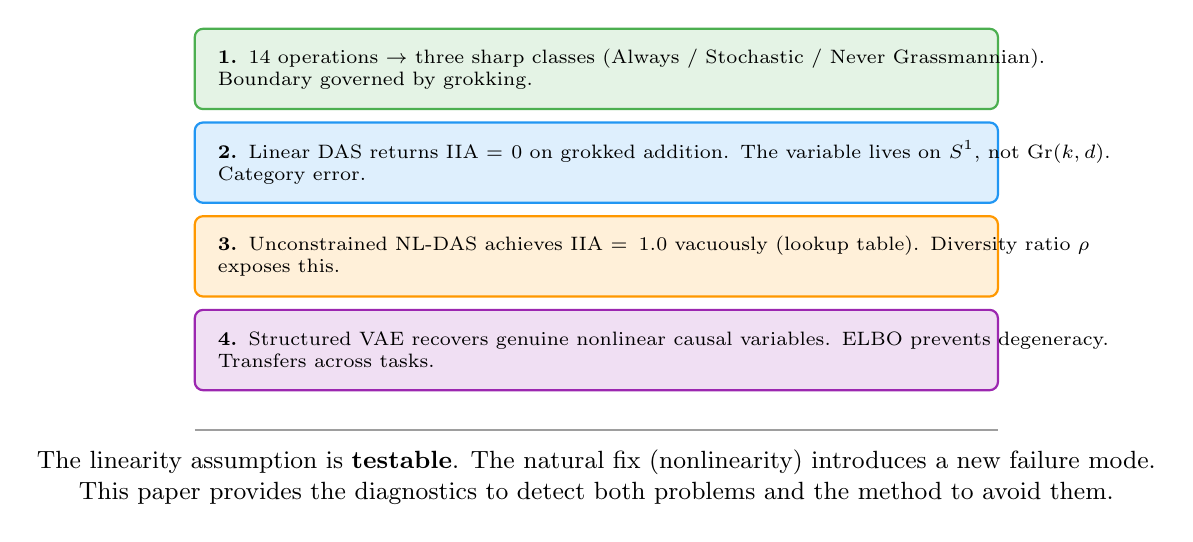
\begin{tikzpicture}[scale=0.85]
  % Finding 1
  \fill[always!15,rounded corners=3pt] (-5.5,3.0) rectangle (6.5,4.2);
  \draw[always,thick,rounded corners=3pt] (-5.5,3.0) rectangle (6.5,4.2);
  \node[font=\scriptsize,align=left,anchor=west,text width=11.5cm] at (-5.3,3.6) {\textbf{1.} 14 operations $\to$ three sharp classes (Always / Stochastic / Never Grassmannian). Boundary governed by grokking.};

  % Finding 2
  \fill[das!15,rounded corners=3pt] (-5.5,1.6) rectangle (6.5,2.8);
  \draw[das,thick,rounded corners=3pt] (-5.5,1.6) rectangle (6.5,2.8);
  \node[font=\scriptsize,align=left,anchor=west,text width=11.5cm] at (-5.3,2.2) {\textbf{2.} Linear DAS returns IIA $= 0$ on grokked addition. The variable lives on $S^1$, not $\Gr(k,d)$. Category error.};

  % Finding 3
  \fill[nldas!15,rounded corners=3pt] (-5.5,0.2) rectangle (6.5,1.4);
  \draw[nldas,thick,rounded corners=3pt] (-5.5,0.2) rectangle (6.5,1.4);
  \node[font=\scriptsize,align=left,anchor=west,text width=11.5cm] at (-5.3,0.8) {\textbf{3.} Unconstrained NL-DAS achieves IIA $= 1.0$ vacuously (lookup table). Diversity ratio $\rho$ exposes this.};

  % Finding 4
  \fill[vae!15,rounded corners=3pt] (-5.5,-1.2) rectangle (6.5,0.0);
  \draw[vae,thick,rounded corners=3pt] (-5.5,-1.2) rectangle (6.5,0.0);
  \node[font=\scriptsize,align=left,anchor=west,text width=11.5cm] at (-5.3,-0.6) {\textbf{4.} Structured VAE recovers genuine nonlinear causal variables. ELBO prevents degeneracy. Transfers across tasks.};

  % Bottom line
  \draw[neutral,thick] (-5.5,-1.8) -- (6.5,-1.8);
  \node[font=\small,align=center] at (0.5,-2.5) {The linearity assumption is \textbf{testable}. The natural fix (nonlinearity) introduces a new failure mode.\\This paper provides the diagnostics to detect both problems and the method to avoid them.};
\end{tikzpicture}
\end{frame}

%% --- SLIDE: The big picture ---
\begin{frame}{The big picture}

\begin{center}
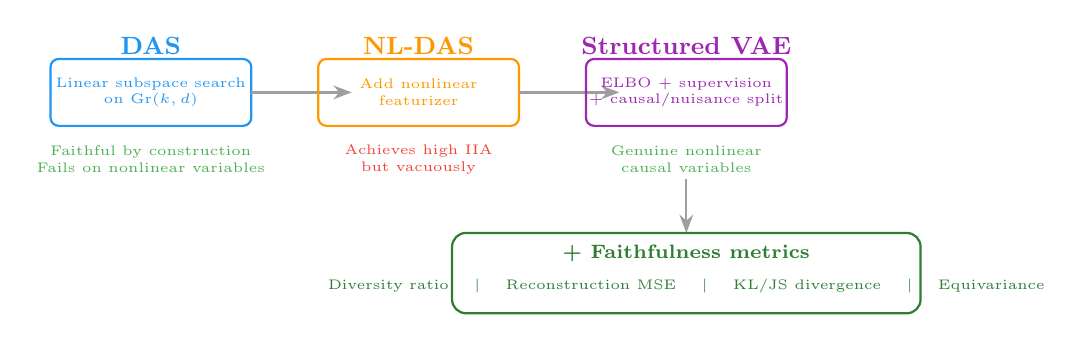
\begin{tikzpicture}[scale=0.85]
  % Timeline / flow
  \node[font=\small\bfseries,das] at (-4,3) {DAS};
  \draw[das,thick,rounded corners=3pt] (-5.5,1.8) rectangle (-2.5,2.8);
  \node[font=\tiny,das,align=center] at (-4,2.3) {Linear subspace search\\on $\Gr(k,d)$};
  \node[font=\tiny,pass,align=center] at (-4,1.3) {Faithful by construction\\Fails on nonlinear variables};

  \draw[neutral,thick,-{Stealth}] (-2.5,2.3) -- (-1,2.3);

  \node[font=\small\bfseries,nldas] at (0,3) {NL-DAS};
  \draw[nldas,thick,rounded corners=3pt] (-1.5,1.8) rectangle (1.5,2.8);
  \node[font=\tiny,nldas,align=center] at (0,2.3) {Add nonlinear\\featurizer};
  \node[font=\tiny,fail,align=center] at (0,1.3) {Achieves high IIA\\but vacuously};

  \draw[neutral,thick,-{Stealth}] (1.5,2.3) -- (3,2.3);

  \node[font=\small\bfseries,vae] at (4,3) {Structured VAE};
  \draw[vae,thick,rounded corners=3pt] (2.5,1.8) rectangle (5.5,2.8);
  \node[font=\tiny,vae,align=center] at (4,2.3) {ELBO + supervision\\+ causal/nuisance split};
  \node[font=\tiny,pass,align=center] at (4,1.3) {Genuine nonlinear\\causal variables};

  % Diagnostics below
  \draw[neutral,thick,-{Stealth}] (4,1.0) -- (4,0.2);
  \draw[grass,thick,rounded corners=5pt] (0.5,-1.0) rectangle (7.5,0.2);
  \node[font=\scriptsize\bfseries,grass] at (4,-0.1) {+ Faithfulness metrics};
  \node[font=\tiny,grass,align=center] at (4,-0.6) {Diversity ratio \quad $|$ \quad Reconstruction MSE \quad $|$ \quad KL/JS divergence \quad $|$ \quad Equivariance};
\end{tikzpicture}
\end{center}

\vspace{0.5em}
\centering
{\small Every causal abstraction claim should be evaluated with the \textbf{four-level hierarchy}.\\IIA is necessary but never sufficient.}
\end{frame}

%% --- SLIDE: Thank you ---
\begin{frame}[plain]
\vfill
\begin{center}
{\Large\bfseries Thank you}

\vspace{1em}
{\small Code and experiments:\\
\texttt{github.com/elliottower/grokking-causal-geometry}}

\vspace{0.5em}
{\small Elliot Tower \quad $\cdot$ \quad Ivan Vegner \quad $\cdot$ \quad N.\ Siddharth \quad $\cdot$ \quad Alex Doumas}

\vspace{1em}
{\small \textcolor{neutral}{Draft paper: \emph{When Does Linear Causal Abstraction Work?\\Mapping the Boundary on the Grassmannian}}}
\end{center}
\vfill
\end{frame}

\end{document}
